\documentclass[11pt,twoside,openright]{report}

\usepackage[algoruled]{algorithm2e}
\usepackage{amsfonts}
\usepackage{amsmath}
\usepackage{amssymb}
\usepackage{bm}
\usepackage{cleveref}
\usepackage{color}
\usepackage{float}
\usepackage{fontspec}
\usepackage{mathpazo}
\usepackage{mathtools}
\usepackage{minted}
\usepackage{wrapfig}
\usepackage{subcaption}
\usepackage[numbers]{natbib}
\usepackage[separate-uncertainty=true]{siunitx}

\usepackage{emptypage}

\usepackage[nottoc]{tocbibind}

\usepackage[intoc, english]{nomencl}
\makenomenclature

\setmonofont[Mapping=tex-text, Scale=0.85]{Menlo}
\usemintedstyle{}

% \usepackage[a4paper, margin=1in]{geometry}
% This is for writing only, so it's easier to read.
\usepackage[paperheight=10.69in,paperwidth=6.87in,tmargin=.4in,bmargin=.6in,inner=.2in,outer=.4in,heightrounded]{geometry}

\renewcommand*{\thefootnote}{(\arabic{footnote})}

\allowdisplaybreaks

%\setmainfont{Palatino Linotype}
% The Palatino package gives a pretty terrible look to the PDF when compiling on
% Windows, so we need to use fontspec instead. Palatino Linotype exists on
% Windows but not on Mac (where Palatino exists instead). So...
\suppressfontnotfounderror1
\def\myfont{Palatino}
\def\myfallback{Palatino Linotype}
\count255=\interactionmode
\batchmode
\font\foo="\myfont"\space at 10pt
\ifx\foo\nullfont
  \font\foo = "\myfallback"\space at 10pt
  \ifx\foo\nullfont
    \errorstopmodep
    \errmessage{no suitable font found}
  \else
    \let\myfont=\myfallback
  \fi
\fi
\interactionmode=\count255
\setmainfont[Ligatures=TeX]{\myfont}

% This will add the units
%----------------------------------------------
\newcommand{\nomunit}[1]{%
\renewcommand{\nomentryend}{\hspace*{\fill}#1}}
%----------------------------------------------


\DeclareSIUnit{\parsec}{pc}

% Define common symbols
\newcommand\balpha{\bm{\alpha}}
\newcommand\bphi{\bm{\phi}}
\newcommand\bvarphi{\bm{\varphi}}

\newcommand\bbA{\mathbb{A}}
\newcommand\bbB{\mathbb{B}}
\newcommand\bbC{\mathbb{C}}
\newcommand\bbD{\mathbb{D}}
\newcommand\bbE{\mathbb{E}}
\newcommand\bbF{\mathbb{F}}
\newcommand\bbG{\mathbb{G}}
\newcommand\bbH{\mathbb{H}}
\newcommand\bbI{\mathbb{I}}
\newcommand\bbJ{\mathbb{J}}
\newcommand\bbK{\mathbb{K}}
\newcommand\bbL{\mathbb{L}}
\newcommand\bbM{\mathbb{M}}
\newcommand\bbN{\mathbb{N}}
\newcommand\bbO{\mathbb{O}}
\newcommand\bbP{\mathbb{P}}
\newcommand\bbQ{\mathbb{Q}}
\newcommand\bbR{\mathbb{R}}
\newcommand\bbS{\mathbb{S}}
\newcommand\bbT{\mathbb{T}}
\newcommand\bbU{\mathbb{U}}
\newcommand\bbV{\mathbb{V}}
\newcommand\bbW{\mathbb{W}}
\newcommand\bbX{\mathbb{X}}
\newcommand\bbY{\mathbb{Y}}
\newcommand\bbZ{\mathbb{Z}}

\newcommand\bA{\mathbf{A}}
\newcommand\bB{\mathbf{B}}
\newcommand\bC{\mathbf{C}}
\newcommand\bD{\mathbf{D}}
\newcommand\bE{\mathbf{E}}
\newcommand\bF{\mathbf{F}}
\newcommand\bG{\mathbf{G}}
\newcommand\bH{\mathbf{H}}
\newcommand\bI{\mathbf{I}}
\newcommand\bJ{\mathbf{J}}
\newcommand\bK{\mathbf{K}}
\newcommand\bL{\mathbf{L}}
\newcommand\bM{\mathbf{M}}
\newcommand\bN{\mathbf{N}}
\newcommand\bO{\mathbf{O}}
\newcommand\bP{\mathbf{P}}
\newcommand\bQ{\mathbf{Q}}
\newcommand\bR{\mathbf{R}}
\newcommand\bS{\mathbf{S}}
\newcommand\bT{\mathbf{T}}
\newcommand\bU{\mathbf{U}}
\newcommand\bV{\mathbf{V}}
\newcommand\bW{\mathbf{W}}
\newcommand\bX{\mathbf{X}}
\newcommand\bY{\mathbf{Y}}
\newcommand\bZ{\mathbf{Z}}
\newcommand\ba{\mathbf{a}}
\newcommand\bb{\mathbf{b}}
\newcommand\bc{\mathbf{c}}
\newcommand\bd{\mathbf{d}}
\newcommand\be{\mathbf{e}}
\newcommand\Bf{\mathbf{f}}
\newcommand\bg{\mathbf{g}}
\newcommand\bh{\mathbf{h}}
\newcommand\bi{\mathbf{i}}
\newcommand\bj{\mathbf{j}}
\newcommand\bk{\mathbf{k}}
\newcommand\bl{\mathbf{l}}
\newcommand\Bm{\mathbf{m}}
\newcommand\bn{\mathbf{n}}
\newcommand\bo{\mathbf{o}}
\newcommand\bp{\mathbf{p}}
\newcommand\bq{\mathbf{q}}
\newcommand\br{\mathbf{r}}
\newcommand\bs{\mathbf{s}}
\newcommand\bt{\mathbf{t}}
\newcommand\bu{\mathbf{u}}
\newcommand\bv{\mathbf{v}}
\newcommand\bw{\mathbf{w}}
\newcommand\bx{\mathbf{x}}
\newcommand\by{\mathbf{y}}
\newcommand\bz{\mathbf{z}}

\newcommand\cA{\mathcal{A}}
\newcommand\cB{\mathcal{B}}
\newcommand\cC{\mathcal{C}}
\newcommand\cD{\mathcal{D}}
\newcommand\cE{\mathcal{E}}
\newcommand\cF{\mathcal{F}}
\newcommand\cG{\mathcal{G}}
\newcommand\cH{\mathcal{H}}
\newcommand\cI{\mathcal{I}}
\newcommand\cJ{\mathcal{J}}
\newcommand\cK{\mathcal{K}}
\newcommand\cL{\mathcal{L}}
\newcommand\cM{\mathcal{M}}
\newcommand\cN{\mathcal{N}}
\newcommand\cO{\mathcal{O}}
\newcommand\cP{\mathcal{P}}
\newcommand\cQ{\mathcal{Q}}
\newcommand\cR{\mathcal{R}}
\newcommand\cS{\mathcal{S}}
\newcommand\cT{\mathcal{T}}
\newcommand\cU{\mathcal{U}}
\newcommand\cV{\mathcal{V}}
\newcommand\cW{\mathcal{W}}
\newcommand\cX{\mathcal{X}}
\newcommand\cY{\mathcal{Y}}
\newcommand\cZ{\mathcal{Z}}

\newcommand\fA{\mathfrak{A}}
\newcommand\fB{\mathfrak{B}}
\newcommand\fC{\mathfrak{C}}
\newcommand\fD{\mathfrak{D}}
\newcommand\fE{\mathfrak{E}}
\newcommand\fF{\mathfrak{F}}
\newcommand\fG{\mathfrak{G}}
\newcommand\fH{\mathfrak{H}}
\newcommand\fI{\mathfrak{I}}
\newcommand\fJ{\mathfrak{J}}
\newcommand\fK{\mathfrak{K}}
\newcommand\fL{\mathfrak{L}}
\newcommand\fM{\mathfrak{M}}
\newcommand\fN{\mathfrak{N}}
\newcommand\fO{\mathfrak{O}}
\newcommand\fP{\mathfrak{P}}
\newcommand\fQ{\mathfrak{Q}}
\newcommand\fR{\mathfrak{R}}
\newcommand\fS{\mathfrak{S}}
\newcommand\fT{\mathfrak{T}}
\newcommand\fU{\mathfrak{U}}
\newcommand\fV{\mathfrak{V}}
\newcommand\fW{\mathfrak{W}}
\newcommand\fX{\mathfrak{X}}
\newcommand\fY{\mathfrak{Y}}
\newcommand\fZ{\mathfrak{Z}}

\usepackage{afterpage}

\renewcommand{\bibname}{References}

\newcommand\blankpage{%
    \null
    \thispagestyle{empty}%
    \newpage}

\newcommand\norm[1]{\left\|#1\right\|}
\newcommand\floor[1]{\left\lfloor#1\right\rfloor}
\newcommand\abs[1]{\left|#1\right|}

\DeclareMathOperator*{\argmax}{argmax}
\DeclareMathOperator*{\argmin}{argmin}
\DeclareMathOperator{\spn}{span}
\DeclareMathOperator{\var}{var}
\DeclareMathOperator{\cov}{cov}
\DeclareMathOperator{\avg}{avg}

\newcommand\jn[1]{{\color{red}(jn: #1)}}

\title{Active Learning with Gaussian Processes\\for Photometric Redshift Prediction}
\author{Jakub Leszek Nabaglo}
\date{October 2017}
\usepackage{layouts}

\pagenumbering{gobble}

\begin{document}
\begin{titlepage}
  \enlargethispage{2cm}
  \begin{center}
    \makeatletter
    \hspace{0pt} \\[3cm]
    \huge\@title \\[.4cm]

    \LARGE\@author \\[8.5cm]
    \makeatother
    \Large A thesis submitted in partial fulfillment of the degree of \\
    \LARGE Bachelor of Philosophy (Honours) -- Science\\[3cm]

    \LARGE Australian National University \\[1cm]
    October 2017
  \end{center}
\end{titlepage}

\vspace*{5cm}
\begin{center}
  Except where otherwise indicated, this thesis is my own original
  work.
\end{center}

\vspace*{2cm}

\hspace{8cm}\makeatletter\@author\makeatother\par
\hspace{8cm}26 October 2017

\vspace*{12cm}

This research made use of Astropy \cite{Astropy} and scikit-learn \cite{Sklearn}.

\begin{center}
  \copyright\ 2017 Jakub Nabaglo
\end{center}
\noindent

\begin{abstract}
  It is expensive to obtain the spectrum needed to accurately calculate the redshift of an astronomical object. We often estimate an object's redshift using cheaper photometric measurements. Spectra are required to generate labels in this regression problem. Large training sets are hence costly, limiting their accuracy and range. Unlabelled samples are abundant. \jn{The sentences don't really follow from each other.}

  We develop a regressor based on Gaussian processes, and apply active learning to select samples for labelling based on their potential for improving the model's accuracy. This permits us to improve redshift predictions at a reduced cost.

  \jn{Mention some concrete results}
\end{abstract}

\cleardoublepage

\renewcommand{\abstractname}{Acknowledgements}
\begin{abstract}
English is not powerful enough to express my gratitude to Cheng Soon Ong. His encouragement propelled me through this year, his questions inspired much contemplation, and the depth of his knowledge never ceased to amaze. I could not have wished for a better supervisor.

On many occasions I encroached on the time of Christian Wolf, whose enthusiasm for astronomy is truly contagious. I always left his office with relevant insight and domain knowledge, the kind of which we often overlook in data science.

I must thank my parents, Ilona and Leszek; my siblings, Agata and Andrew; and my girlfriend Lily. They supported me through many years of study, and through the peaks and valleys of life.

Finally, I am indebted to Matthew Alger, for his advice, careful proofreading, and assistance taming truculent software.
\end{abstract}

\thispagestyle{empty}

\pagenumbering{arabic}

\addtocounter{page}{5}
\tableofcontents

\nomenclature{$\cX$}{Predictor input space}
\nomenclature{$\bbR$}{Set of real numbers}
\nomenclature{$\bbR_{\geq0}$}{Set of non-negative real numbers}
\nomenclature{$f$}{Original function}
\nomenclature{$\hat f$}{Predictor}
\nomenclature{$n$}{\jn{fill}}
\nomenclature{$m$}{\jn{fill}}
\nomenclature{$d$}{\jn{fill}}
\nomenclature{$c$}{Speed of light in a vacuum\nomunit{\SI{299792458}{\meter\per\second}}}
\nomenclature{$z$}{Redshift}
\nomenclature{$\cP$}{Powerset}
\nomenclature{$\cY$}{Predictor output space}
\nomenclature{$z_\mathrm{spec}$}{Spectroscopic redshift}
\nomenclature{$z_\mathrm{pred}$}{Photometric redshift}
\nomenclature{$\fF$}{Space of predictors}
\nomenclature{$\fD$}{Space of training sets}
\nomenclature{$\cE$}{Space of error functions}


\printnomenclature


\chapter{Introduction}

A redshift is the change in the wavelength of a photon emitted by an object that is moving away from the observer. When applied to the visible spectrum, a redshift makes an object appear more red.

Redshifts are important in astronomy, as they are used for a variety of tasks. The most important of these tasks is finding distances to objects.

Currently, redshifts are found using specroscopy. A spectroscope is applied to a galaxy, and its spectral profile is measured. From these measurements, we can isolate the hydrogen lines, which are then compared against the baseline to obtain the redshift. This method is problematic as it requires a spectroscope to be pointed at each galaxy whose redshift we wish to measure. Since there are many galaxies in the universe, it is impossible to use this method for large extents of the sky.

Instead, we can utilise a technique called `photometric redshift' prediction. A photometric redshift is one computed from photometric measurements, as opposed to spectroscopic ones. Photometric measurements `bucket' the spectrum into a small number of distinct intervals, much like a photographic camera buckets the visible spectum into red, green, and blue. These buckets can then be used as input to a regressor, and the redshift can be predicted.

Photometric have their own disadvantages. Currently, they only cover a limited range of redshifts. Further, they tend to rely on limited datasets, whose spectra have been measured without much regard to the impact of the sample on the prediction.

It therefore is appropriate to apply optimal design techniques to the problem. Optimal design allows us to choose, from a pool of unlabelled galaxies (i.e., galaxies for which we know the photometric data, but not the exact redshift from spectroscopic data), the one that would bring the most value to the regression problem if it were labelled. In other words, towards which galaxy should we point the spectroscope next so as to give us the most new information?

This method of selection of new training samples has advantages of greater cost effectiveness. It will also permit us to increase the range of current photometric redshift models with the lowest effort.

Optimal design requires us to be able to assess the uncertainties in the prediction for each point in the input space. This provides a useful heuristic for choosing the next sample to label.

\section{Redshift}
  Redshift is a property of all signals we observe from astronomical objects. It is often not easy to measure, but finding it permits us to learn important facts about the object being observed.

  \jn{Caused not just by doppler effect. Also expansion of the universe.}

  The electromagnetic waves that we observe from distant objects are subject to the Doppler effect. This is the phenomenon by which waves produced by an object that is moving away from the observer appear to have a longer wavelength. Consider an ambulance driving away from you: the tone of the siren appears lower than if the ambulance was stationary. In a similar way, a galaxy moving away from us appears redder, giving rise to the term `redshift'. The converse effect, affecting objects moving towards the observer, is termed `blueshift'.

  The redshift of an object is then directly correlated to its velocity perpendicular to the line of sight from the observer. For a redshift $z$, the line-of-sight velocity is\[
      v \approx cz \text{,}
  \] where $c$ is the speed of light constant.

  This permits us to approximate the distance from the observed object. Due to the expansion of space, distant objects are moving away from us at a velocity proportional to their distance. For a velocity $v$, that distance is \[
      D \approx \frac{v}{H_0} \text{,}
  \] where $H_0$ is the Hubble parameter, equalling approximately $\SI{70}{\kilo\meter\per\second\per\mega\parsec}$. For faraway objects then, the redshift is hence proportional to distance.

  Since the speed of light is finite, electromagnetic waves coming from distant objects represent the past. Hence, observing distant objects permits us to study the history of the universe. For example, the universe is denser at larger distances, as a remnant of the earlier stages of the big bang. Similarly, large distances contain more quasars and more brighter objects. The ability to compute distance from the redshift is important in studying the past of the universe as the distance is a proxy for the age of the object we observe.

  The mass of an object is correlated to its luminosity\footnote{The luminosity is its total amount of light emitted.}. The luminosity can be approximated from the brightness using the object's distance. Hence, computing the distance of an object from the redshift permits us to approximate its size.

  However, for some objects, we can approximate the size more directly. For closer objects, we can measure their apparent radius as the angle they span on the sky. Using trigonometry, we can then compute the actual radius of such an object from its apparent radius and redshift-derived distance.

  For closer galaxies, we are able to observe the movements of stars inside the galaxy. When a star orbits the centre of a galaxy, the internal motion can cancel or amplify the star's line-of-sight velocity. Measuring the stars' velocities from redshift hence permits us to to study galaxy dynamics.

\chapter{Photometry}

  \begin{figure}
    \centering
    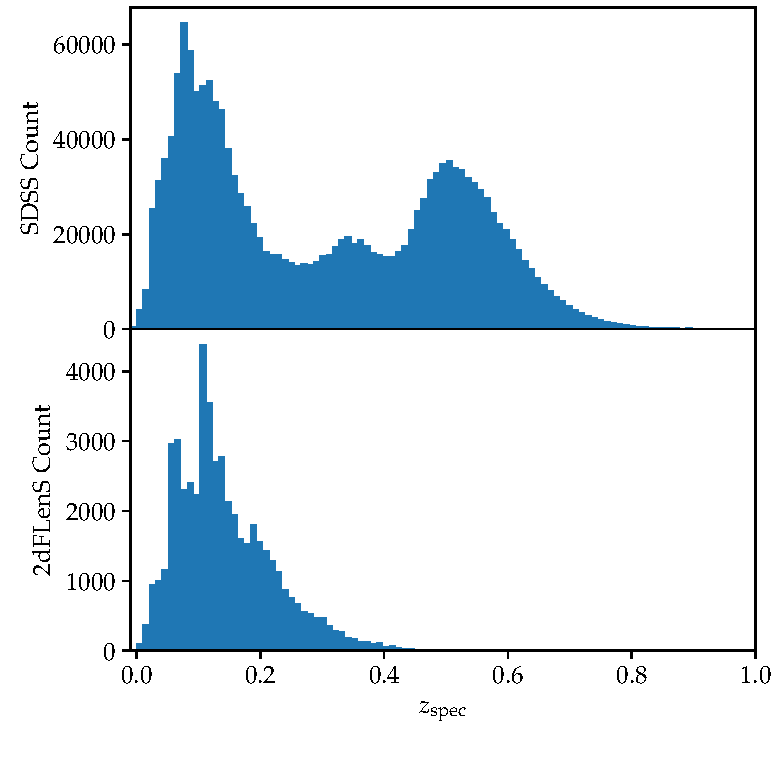
\includegraphics[width=0.9\textwidth]{zpec_hist.pdf}
    \caption{Histogram of objects in SDSS and 2dFLenS by spectroscopic redshift.}
    \label{fig:spec_hist}
  \end{figure}

  Photometry is a technique in astronomy, where we measure the amount of light that reaches a telescope from an object. The wavelength information is ignored, although filters may be used to discard some light, giving us limited wavelength information. \jn{cite something}

  Photometry is analogous to digital photography. Our cameras use three filters (red, green, and blue) to separate colour information. They then measure he amount of light reaching the sensor. After processing, they yield three colour values per pixel. \jn{cite something?}

  Spectroscopy is a related technique that not only measures the amount of received, but also measures its wavelength. This yields a full spectrum of the object, instead of a few colours. It is used to accurately compute the redshift of an object: the spectra of distant objects are compared to those of nearby objects, and the offset between them is the redshift. \jn{cite}

  However, spectroscopy is expensive since a telescope can only measure the spectrum of a few objects at a time. \jn{cite} This would make it extremely time-consuming to survey the huge number of galaxies in the universe. More distant objects are particularly neglected since light conforms to the inverse square law, so it takes four times longer to measure the spectrum of an object that is twice as far away.

  \section{Colours}

  The amount of light we receive from an object $A$ is its \emph{intensity} $I_A$. Its units are power per area, but we usually measure it in a logarithmic scale called the \emph{apparent magnitude}. The apparent magnitude $m_A$ of an object $A$ is measured relative to the apparent magnitude of Vega, defined to be $0$. An $100$-fold increase in the intensity of an object results in a magnitude that is lower by $5$: for objects $A$ and $B$,\[
    m_A - m_B = -5 \log_{100} \left( \frac{I_A}{I_B} \right) \text.
  \] Counterintuitively, brigter objects have a lower magnitude. The sun has an apparent magnitude of $-27$ and is the brightest object in the sky. \jn{cite}

  We use filters to separate light coming from different sections of the visible light spectrum. In our datasets, these are $u$, $g$, $r$, $i$, and $z$\footnote{In astronomy, $z$ can refer either to an object's redshift or to the infrared band. The meaning of any particular $z$ should be clear from context.}, in increasing order of wavelength. The $u$ band is ultraviolet, $g$ and $r$ are visible, and $i$ and $z$ are infrared. These five filters have a large spread, providing information about objects' emissions in a wide part of the spectrum.

  \jn{a pic of the filters would be nice}

  We use pairwise differences of magnitudes in these bands as the \emph{colours} in photometric redshifts. The colours are $m_u - m_g$, $m_u - m_r$, $m_r - m_i$, and $m_i - m_z$. \jn{cite where they are used} Since the magnitude is a logarithmic scale, for bands $a$ and $b$, $m_a - m_b$ is proportional to $I_b / I_a$, making the colours independent of the apparent magnitude of the object as a whole. In addition to the four colours, we use $m_r$ as a proxy for the apparent magnitude of the object.

  \section{Datasets}
  To predict photometric redshifts, we need a dataset of example objects. For each, we must know the five photometric bands, as well as the spectroscopic redshift. Uncertainty bounds for the photometric data and the redshift are very common, but not used in our model.

  Many suitable datasets exist. The Sloan digital sky survey (SDSS) is very common, and contains a very large number of objects. The 2-degree Field Lensing Survey (2dFLenS) is another dataset we use, with far fewer objects. They have different distributions and cover different ranges of redshifts and magnitudes, permitting us to study the behaviour of our model under differing distributions of data.

  \subsection{Sloan digital sky survey}
  The Sloan digital sky survey (SDSS) is a large photometric and spectroscopic survey of the Northern sky. As of its twelfth data release, it contains useful spectroscopic redshifts for \SI{4266444}{} objects, including \SI{2401952}{} galaxies, along with the corresponding photometric measurements. \citep{SDSS} Of these galaxies, we select those with a redshift uncertainty of less than $0.1$, leaving us with \SI{1707233}{} examples.

  The spectroscopic redshift distribution of objects in SDSS is presented in \cref{fig:spec_hist}. We see that it covers redshifts from about $z_\mathrm{spec} = 0.05$ to about $z_\mathrm{spec} = 0.8$, with some examples existing outside these bounds.

  \jn{a plot of magnitudes $r$ would be nice}

  \jn{a plot of magnitudes $r$ vs $z$ would be nice}

  \subsection{The 2-degree field lensing survey}
  The 2-degree field lensing survey (2dFLenS) is also a photometric and spectroscopic survey. Unlike SDSS, it observes the Southern sky. It lists \SI{50919}{} examples with spectroscopic redshifts and photometric measurements, which is significantly fewer than SDSS.

  The spectroscopic redshift distribution of objects in 2dFLenS is presented in \cref{fig:spec_hist}. Its data spans from about from about $z_\mathrm{spec} = 0.05$ to about $z_\mathrm{spec} = 0.3$, with limited examples existing outside this interval. This is a lower spread than SDSS.

  \jn{a plot of magnitudes $r$ would be nice}

  \jn{a plot of magnitudes $r$ vs $z$ would be nice}

\chapter{Regression on photometric redshifts}

Given some spectroscopic labels, we wish to find redshifts from photometric data. This problem can be modelled using regression. We introduce regression and develop a predictor for photo-$z$ and report its performance. We then extend regression to Gaussian processes, a family of models capable of reporting their confidence in their own predictions. These are later used in active learning to lower the number of spectra required to further improve our accuracy.

To formalise regression, let $\cX \subset \bbR^d$ and $\cY \subset \bbR$ both be bounded. Let $f$ map $\cX$ to $\cY$. We are given a set \[
  \cD = \left\{\left(\bx_1, y_1\right), \dots, \left(\bx_n, y_n\right)\right\}
\] of $n$ \emph{samples} of $f$, where $y_1, \dots, y_n$ are the \emph{labels}. Let $h$ be the probability distribution of the label noise. Then for all $i$, \[
  y_i = f(\bx_i) + \epsilon \text{ for some error } \epsilon \sim h \text{.}
\] Regression is the task of reconstructing $f$ from the finitely many examples of its inputs and outputs we have. $\cD$ is the \emph{training set}. Define $\fD \subset \cP(\cX \times \cY)$ to be the space of possible training sets.

In our case, $\cX$ is the space of photometric measurements that contains our input samples, and $\cY \subset (-1, \infty)$ is the space of redshifts spanned by our labels. Let $f$ is the physical function that maps photometric measurements to redshifts. Since it is physically possible to have two objects with the same photometry but different redshifts, it is not obvious why it is valid to assume that such a function exists. To resolve this, we let $f$ be the function that maps photometric measurements to to any corresponding object's \emph{most likely} redshift. This lets us treat any inconsistency as any other source of noise.

To solve a regression problem, let $\hat\cF$ be our space of approximations that we consider; its exact membership depends on our assumptions. A function $F : \fD \to \hat\cF$ is our \emph{model}. Given a training set, it returns a predictor; this is referred to as \emph{training} the model. Define $\hat f \coloneqq F(\cD)$ to be our predictor.

We want to find $\hat f \in \hat\cF$ that is the best approximation of $f$. Each candidate approximation $\hat f_c \in \hat\cF$ can be assigned a likelihood that quantifies how good an approximation it is:\[
    p\left(\hat f_c \;\middle|\; \cD \right) \text{.}
\] We define $\hat f$ to be the function that maximises this likelihood:\[
    \hat f = F(\cD) \coloneqq \argmax_{\hat f_c \in \cF} p\left(\hat f_c \;\middle|\; \cD \right) \text{.}
\] The definition of this likelihood depends on our assumptions about $f$, $h$, and $F$.

In our specific case we always assume that the noise is distributed according to a Gaussian with a $0$ mean and a with variance $\sigma^2$ that we leave as a hyperparameter\footnote{A hyperparameter is a parameter that depends on the distribution of our data.}.

Some models are capable of not only predicting $f$ but also returning a measure of their confidence in their own prediction. Gaussian process regression (GPR) is an example of such a model. This measure of confidence becomes crucial when we seek to improve our predictions with active learning.

\section{Assessing performance}

To assess the performance of a model, we must have a way of quantifying its accuracy. We withhold a portion of our data into a \emph{testing set} $\cD' \in \fD$ that is disjoint from $\cD$. Let $n' \coloneqq \abs{\cD'}$ and index the elements\[
  \cD' = \{(\bx'_1, y'_1), \dots, (\bx'_{n'}, y'_{n'})\}
\].

For each $i = 1, \dots, n'$ define the prediction as\[
  \hat y'_i \coloneqq \hat f(\bx'_i) \text{.}
\] Define the $\delta z$ error as \[
  \delta z_i \coloneqq \hat y'_i - y'_i\text,
\] as used in \citep{SDSSPhotoZ} and \citep{Chris}. For redshifts, define $dz$ as \[
  dz_i \coloneqq \frac{\delta_i}{1 + y'_i} \text.
\] This accounts for the physical significance of the redshift: $1 + z$ is the ratio of the size of the universe when the light was emitted to its size now. \jn{citation} Then $dz_i$ is proportional to the resulting error when we use our predictions to calculate the historical size of the universe.

For a perfect predictor,\[
  \hat y'_i = y'_i \text{ for all }i=1, \dots, n'\text{,}
\] so $\delta_i = 0$. Unfortunately, perfect predictors are rarely possible to produce. This is due to our fundamental ability to reconstruct an arbitrary function from a finite number of samples\footnote{The space $\cF$ of functions $\cX \to \cY$ has a higher cardinality than the space $\fD$ of training sets. Any given model $F$ is thus not bijective. Therefore there exists a function $f \in \cF$ that cannot be approximated by $F$ from a finite dataset in $\fD$.}. Even knowing the form of $f$, noise label will reduce the accuracy of our predictor.

There exist many scores that permit us to compare predictors. The fraction of variance unexplained is a commonly used score. Others, more specific to photometric redshifts, are the mean $dz$ error, the $dz$ deviation, and the fraction of $dz$ outliers. Photometric redshifts suffer from a high number of outliers; their influence is reduced with these redshift-specific scores.

\subsection{Fraction of variance unexplained}
The fraction of variance unexplained (FVU) measures the fraction of the variance of the labels $y'_1, \dots, y'_{n'}$ not explained by the predictor.

To define it, let $\mathrm{VAR_{err}} \coloneqq \frac{1}{n'}\sum_{i=1}^{n'}\delta_i^2$ be the mean squared $\delta$ error. If the mean $\delta$ error is zero, this equals the variance\footnote{For a finite set $S = \{s_1, \dots, s_{\abs{S}}\} \subset \bbR$ of $\abs{S}$ elements, we define the variance as $\var S \coloneqq \frac1{\abs{S}}\sum_{i=1}^{\abs{S}}(s_i - \overline{s})^2$, where $\overline{s} \coloneqq \frac1{\abs{S}}\sum_{i=1}^{\abs{S}}s_i$ is the mean of $S$.} of the $\delta$ errors. Let $\mathrm{VAR_{tot}} \coloneqq \var\{y'_1, \dots, y'_{n'}\}$ be the variance of the labels of the testing set. Note that $\mathrm{VAR_{err}}$ varies with the predictor, whereas $\mathrm{VAR_{tot}}$ is constant for each testing set. We define \[
  \mathrm{FVU} \coloneqq \frac{\mathrm{VAR_{err}}}{\mathrm{VAR_{tot}}} \text{.}
\]

Values of $\mathrm{FVU}$ closer to $0$ are better. Intuitively, a perfect predictor explains the entire variance of the labels, so we expect it to yield $\mathrm{FVU} = 0$. Indeed, a perfect predictor has $\delta_1 = \dots = \delta_{n'} = 0$, so $\mathrm{VAR_{err}} = 0$. For a predictor that always returns the mean of the testing set, $\mathrm{VAR_{err}} = \mathrm{VAR_{tot}}$ by definition, so $\mathrm{FVU} = 1$, as expected since a predictor that always returns the mean explains none of the variance. A predictor with $\mathrm{FVU} > 1$ then performs worse by our metric than a predictor that always returns the mean.

\subsection{Mean $dz$ error}
The mean $dz$ error is specific to photometric redshifts. It is defined as the mean of all absolute $dz$ errors:\[
  \textrm{mean $dz$ error} \coloneqq \avg\{\abs{dz_1}, \dots, \abs{dz_{n'}}\} \text.
\] Values closer to $0$ are better.

Unlike the fraction of variance unexplained error, which computes the sum of squared errors, the mean $dz$ error depends on a sum of absolute errors (it is a weighted $\ell_1$ loss). This is an important distinction, as the sum of squared errors is more likely to be overly influenced by outliers.

\subsection{$dz$ bias}

The $dz$ bias is also specific to photometric redshifts. It quantifies whether the predictor is more likely to over- or underestimate the redshift. It is defined as to be the mean of all signed $dz$ errors:\[
  \textrm{$dz$ bias} \coloneqq \avg\{ dz_1, \dots, dz_{n'} \} \text.
\] Unlike the FVU and the mean $dz$ error, the $dz$ bias is permitted to be negative. In addition, a $dz$ bias of zero, whilst desirable, does not indicate a perfect predictor.

\subsection{$dz$ deviation}

The $dz$ deviation is defined as the half-width of the deviation of $dz$ containing $68.3\%$ of all objects. More formally, the $dz$ deviation is the smallest $\sigma \in \bbR_{\geq0}$ such that $68.3\%$ of $dz_i$ errors are within $[-\sigma, \sigma]$. It has the advantage of completely discarding outliers beyond percentile $68.3$, vastly reducing their influence.

\subsection{Fraction of $dz$ outliers}

The fraction of $dz$ outliers is defined as the fraction of objects with $\abs{dz} > 0.1$. It quantifies the fraction of objects whose redshifts fail to be explained by the model.

\section{Existing methods}

\jn{write intro to section}

\jn{cite Chris' paper heavily}

\subsection{Kernel density estimation}

\jn{Write about Chris's KDE}

\subsection{Neural networks}

\jn{write}

\subsection{Boosted decision trees}

\jn{Boosted decision trees}

\subsection{Template methods}

\jn{write}

\section{Linear regression}
  \begin{wrapfigure}{R}{0.4\textwidth}
    \centering
    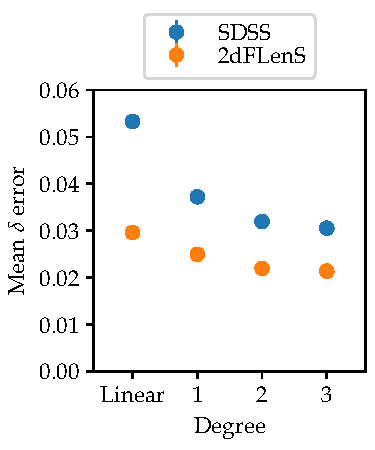
\includegraphics[width=0.4\textwidth]{linreg_polynomial.pdf}
    \caption{Error of linear regression with polynomial features. Note that degree 1 polynomial features are equivalent to linear regression with a bias term.}
    \label{fig:linreg_polynomial}
  \end{wrapfigure}

Linear regression is a simple regression model that expresses $\hat f(\bx)$ as a fixed linear combination of the components of $\bx$.

More formally, we suppose that \[
  \hat f(\bx) = \bx^\top\bw \text.
\]

We assume that $p(\hat f \mid \cD)$ depends only on how well $\hat f$ approximates $f$ at the training samples. Assuming Gaussian likelihoods with variance $\sigma^2$, we wish to find $\bw$ that yields the best predictor. We derive the least squares error.

By our assumption of Gaussian likelihoods, \begin{align}
    p\left(\hat f \;\middle|\; \cD\right) &= \prod_{i = 1}^{n} \cN\left(\hat y_i \;\middle|\; y_i, \sigma^2\right) \label{eq:linearlikelihood} \\
    &= \prod_{i = 1}^{n} \frac{1}{\sqrt{2\pi\sigma^2}} \exp\left(-\frac{\left(\hat y_i - y_i\right)^2}{2\sigma^2}\right) \text. \nonumber
\end{align} We wish to find $\bw$ that maximises this likelihood. This is equivalent to minimising the negative log likelihood:\begin{align*}
    -\log p\left(\hat f \;\middle|\; \cD\right)
    &= - \sum_{i = 1}^{n} \log\left[\frac{1}{\sqrt{2\pi\sigma^2}} \exp\left(-\frac{\left(\hat y_i - y_i\right)^2}{2\sigma^2}\right)\right] \\
    &= - \sum_{i = 1}^{n} \left(-\frac{1}{2}\log\left(2\pi\sigma^2\right) -\frac{\left(\hat y_i - y_i\right)^2}{2\sigma^2}\right) \\
    &=  \frac{n}{2}\log\left(2\pi\sigma^2\right) + \frac{1}{2\sigma^2}\sum_{i = 1}^{n}\left(\hat y_i - y_i\right)^2 \text{.}
\end{align*} Since $\frac{n}{2}\log(2\pi\sigma^2)$ and $1/\sigma^2$ are constant, minimising the negative log likelihood is equivalent to minimising $\frac{1}{2\sigma^2}\sum_{i = 1}^{n}(\hat y_i - y_i)^2$. We call this our \emph{loss} function and write \[
  E(\bw) \coloneqq \frac{1}{2\sigma^2}\sum_{i = 1}^{n}\left(\hat y_i - y_i\right)^2 \text.
\] This is called the \emph{sum of squares} loss. Note that we can compute it without knowing $\sigma^2$.

 minimising $-\log p(\by \mid \hat f, X)$ is equivalent to minimising $\frac{1}{2\sigma^2}\sum_{i = 1}^{n}(\hat y_i - y_i)^2$. Further, since $1/\sigma^2$ is constant, this is equivalent to minimising $\frac12\sum_{i = 1}^{n}(\hat y_i - y_i)^2$.

The optimal weights vector is given by \[
    \argmax_{\bw \in \bbR^d} p\left(\hat f \;\middle|\; \cD\right) = \argmin_{\bw \in \bbR^d} E(\bw) \text{.}
\]

We can solve this analytically. We rewrite \[
  E(\bw) = \frac12(X\bw - y)^\top(X\bw - y) \text,
\] where $X \in \bbR^{n\times d}$ such that $X_i \coloneqq \bx_i$. Setting the derivative to zero to find the minimum, \[
    \frac{dE(\bw)}{d\bw} = X^\top (X\bw - \by) = \mathbf{0} \text{.}
\] The minimum is \[
    \bw  = \left(X^\top X\right)^{-1}X^\top\by \text.
\]

\subsection{Feature differences}

We show that creating new features that are pairwise differences between existing features does not affect a linear model since the same predictor will be found using the original features. This means that, for a purely linear model, our feature space of photometric colours is equivalent to that of photometric magnitudes.

Let $\bx \in \cX$ and let $D \in \bbR^{d \times d}$ be the matrix of pairwise differences:\[
    D_{ij} \coloneqq x_i - x_j \text{.}
\]

Let $\balpha \in \bbR^d$ be a weights vector for $\bx$ and let $\cB \in \bbR^{d\times d}$ be a weights matrix for $D$. Define our predictor as\[
    \hat f(\bx) = \balpha \cdot \bx + \langle \cB, D \rangle_\mathrm{F} \text{,}\label{eq:pred1}\tag{$*$}
\] where $\langle \cdot, \cdot \rangle_\mathrm{F}$ is the Frobenius inner product.

Let $\tilde\balpha \in \bbR^d$ be defined by \[
    \tilde\balpha_i \coloneqq \balpha_i + \sum_{j=1}^n \cB_{ij} - \sum_{j=1}^n \cB_{ji} \text{.}
\] We show that a predictor defined as \[
    \tilde f(\bx) = \tilde{\balpha} \cdot \bx
\] is equivalent to \eqref{eq:pred1}.

We have that\begin{align*}
    \tilde\balpha \cdot \bx &= \sum_{i=1}^n \bx_i\left( \balpha_i + \sum_{j=1}^n \cB_{ij} - \sum_{j=1}^n \cB_{ji} \right) \\
    &= \sum_{i=1}^n \bx_i\balpha_i +  \sum_{i=1}^n \sum_{j=1}^n \bx_i \cB_{ij} - \sum_{i=1}^n \sum_{j=1}^n \bx_i \cB_{ji} \\
    &= \sum_{i=1}^n \bx_i\balpha_i +  \sum_{i=1}^n \sum_{j=1}^n \bx_i \cB_{ij} - \sum_{i=1}^n \sum_{j=1}^n \bx_j \cB_{ij} \\
    &= \balpha\cdot\bx +  \sum_{i=1}^n \sum_{j=1}^n \cB_{ij} \left(\bx_i - \bx_j \right) \\
    &= \balpha\cdot\bx + \langle \cB, D \rangle_\mathrm{F}
\end{align*} as desired.

Note that this does not apply to models where a nonlinear transformation is applied to $D$. It also does not necessarily hold when regularisation is applied to the weights.

\subsection{Nonlinear features}

\jn{TODO: write}

\section{Kernels}

A kernel is a function $k : \bbR^d \times \bbR^d \to \bbR$ such that \[
    k(\bx, \bx') = \langle \bvarphi\left(\bx\right), \bvarphi\left(\bx'\right)\rangle \text{,}
\] where $\bvarphi : \bbR^d \to H$ maps our feature space $\bbR^d$ to a real Hilbert space $H$. Intuitively, we can think of a kernel as an inner product in a different space.

Kernels permit us to generalise our earlier basis transformations $\bphi : \bbR^d \to \bbR^m$ to $\bvarphi : \bbR^d \to H$. Due to the possibly infinite-dimensional nature of $H$, we cannot use $\bvarphi$ directly. Instead, we can take advantage of it by computing $k$.

Like other inner products, a kernel can be thought of as a similarity measure. For example, $k(\bx, \bx') = 0$, then $\bx$ and $\bx'$ are orthogonal in $H$, and thus not similar at all by our metric.

\subsection{Examples of kernels}
\begin{figure}
  \centering
  \begin{subfigure}{0.5\textwidth}
    \centering
    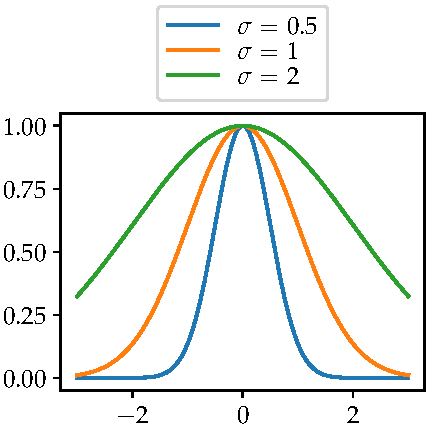
\includegraphics[width=0.9\textwidth]{gaussian_kernel_plot.pdf}
    \caption{$k(0, x)$, where $k$ is the Gaussian kernel.}
    \label{fig:gaussian_kernel}
  \end{subfigure}%
  \begin{subfigure}{0.5\textwidth}
    \centering
    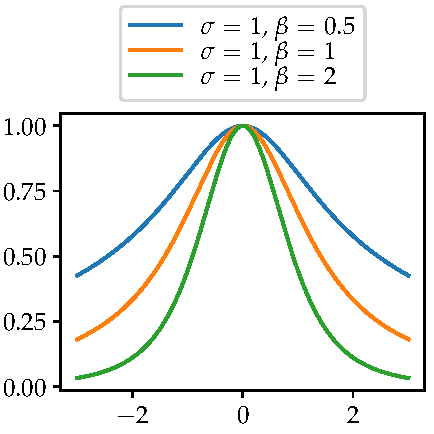
\includegraphics[width=0.9\textwidth]{rational_quadratic_kernel_plot.pdf}
    \caption{$k(0, x)$, where $k$ is the Rational-Quadratic kernel.}
    \label{fig:rational_quadratic_kernel}
  \end{subfigure}
  \begin{subfigure}{0.5\textwidth}
    \centering
    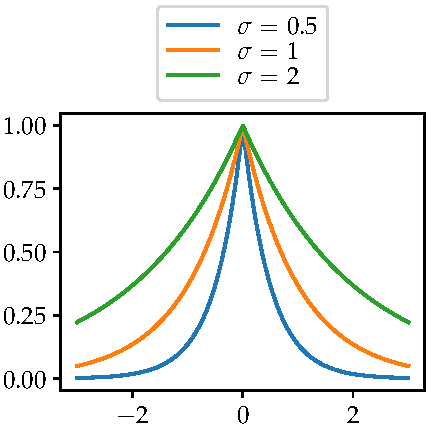
\includegraphics[width=0.9\textwidth]{exponential_kernel_plot.pdf}
    \caption{$k(0, x)$, where $k$ is the Exponential kernel.}
    \label{fig:exponential_kernel}
  \end{subfigure}%
  \begin{subfigure}{0.5\textwidth}
    \centering
    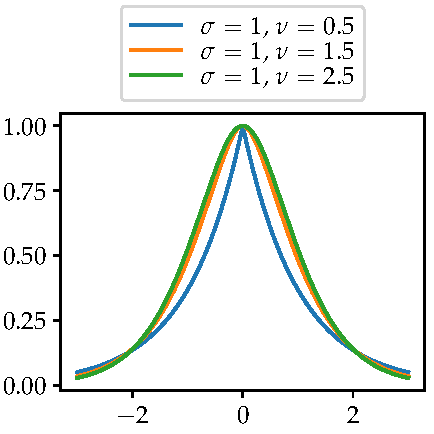
\includegraphics[width=0.9\textwidth]{matern_kernel_plot.pdf}
    \caption{$k(0, x)$, where $k$ is the Mat\'ern kernel.}
    \label{fig:matern_kernel}
  \end{subfigure}
  \caption{Plots of kernels.}
\end{figure}


\subsubsection{Gaussian kernel}

The Gaussian kernel, also known as the radial basis function (RBF) kernel, is very common. Its smoothness is very desirable for many applications and its shape resembles distributions of much real-world data. It is defined by \[
    k(\bx, \bx') \coloneqq \exp\left( - \frac{\norm{\bx - \bx'}^2}{2\sigma^2} \right) \text{,}
\] where the hyperparameter $\sigma$ is known as the \textit{length scale}. This is visualised in \cref{fig:gaussian_kernel}.

An more general definition involves $d$ separate length scales $\sigma_1, \dots, \sigma_d$, permitting us to set the length independently for each dimension. This definition is \[
    k(\bx, \bx') \coloneqq \exp\left( - \frac{1}{2}\left(\bx - \bx'\right)^\top\Sigma^{-1}\left(\bx - \bx'\right) \right) \text{,}
\] where \[
    \Sigma = \begin{bmatrix}
        \sigma_1^2 & & \makebox(0,0){\text{\huge0}} \\
        & \ddots & \\
        \mbox{\huge 0} & & \sigma_d^2
    \end{bmatrix} \text{.}
\]

\subsubsection{Rational-quadratic kernel}

The Rational-quadratic kernel is defined by \[
    k(\bx, \bx') \coloneqq \left(1 + \frac{1}{2\sigma}\norm{\bx - \bx'}^2\right)^{-\beta} \text{,}
\] where $\sigma > 0$ is the \textit{length scale} and $\beta > 0$ is the \textit{shape parameter}. It is a reasonable approximation of the Gaussian kernel that does not require an exponentiation. It is shown in \cref{fig:rational_quadratic_kernel}.

Setting $\sigma = \beta \sigma_0$ and limiting $\beta \to \infty$ yields a Gaussian kernel with length scale $\sigma_0$.

\subsubsection{Exponential kernel}

  The exponential kernel is less common as it is not differentiable, limiting its usefulness to many models. Its definition is \[
    k(\bx, \bx') \coloneqq \exp\left( - \frac{\norm{\bx - \bx'}}{\sigma} \right) \text{,}
  \] where $\sigma > 0$. It is plotted in \cref{fig:exponential_kernel}.


\subsubsection{Mat\'ern kernel}

For some $\bx$ and $\bx'$, define $d \coloneqq \norm{\bx - \bx'}$. The Mat\'ern Kernel is defined by \[
    k(\bx, \bx') \coloneqq \frac{2^{1-\nu}}{\Gamma(\nu)}\left(\frac{\sqrt{2\nu}d}{\sigma}\right)^\nu K_\nu\left(\frac{\sqrt{2\nu}d}{\sigma}\right)
\]$K_\nu$ is the modified Bessel function of the second kind, $\Gamma$ is the Gamma function, $\nu > 0$ is a hyperparameter, and $\sigma > 0$ is the length scale. It is differentiable $\floor{\nu-1}$ times. See \cref{fig:matern_kernel} for a visualisation.

For some values of $\nu$ it can be simplified. When $\nu = 1/2$,
 \[
   k(\bx, \bx') = \exp\left(-\frac{d}{\sigma}\right) \text{;}
 \] when $\nu=3/2$, \[
   k(\bx, \bx') = \left(1 + \frac{\sqrt{3}d}{\sigma}\right)\exp\left(-\frac{\sqrt{3}d}{\sigma}\right) \text{;}
 \] and when $\nu = 5/2$,\[
  k(\bx, \bx') = \left(1 + \frac{\sqrt{5}d}{\sigma} + \frac{5d^2}{3\sigma^2}\right)\exp\left(-\frac{\sqrt{5}d}{\sigma}\right) \text.
 \] For $\nu=1/2$, this kernel the exponential kernel. The other two expressions are an exponential kernel multiplied by a polynomial in $d/\sigma$.

\subsection{Kernel Approximations}

For large dataset, computing $K$ becomes expensive it as has a space complexity of $O(n^2)$.

\subsubsection{RBF sampling}

RBF Sampling approximates the Gaussian kernel by sampling from its Fourier transform. \jn{I literally don't know if this is correct}

\jn{prove}

\subsubsection{Empirical kernel map}

\jn{TODO: WRITE}


\subsection{Kernelised linear regression}

  \begin{wrapfigure}{R}{0.4\textwidth}
    \centering
    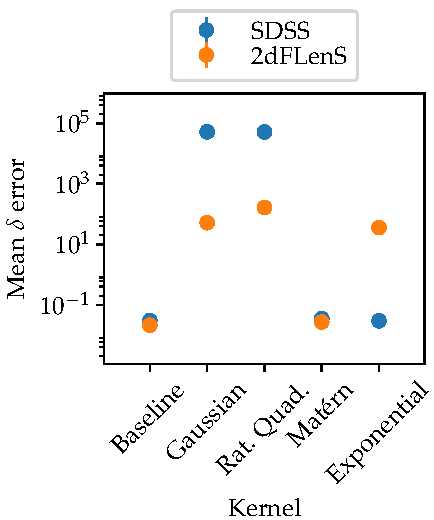
\includegraphics[width=0.4\textwidth]{linreg_kernelised.pdf}
    \caption{Error of kernelised linear regression. The $\sigma$ is the median distance between training $\bx$ values.}
    \label{fig:linreg_kernelised}
  \end{wrapfigure}

To extend our range of possible feature maps, we rewrite linear regression to use kernels. Let $\bphi : \bbR^{d} \to \bbR^{d'}$ be our feature map.

Recall that the loss function $E : \bbR^{d'} \to \bbR_{\geq0}$ that we wish to minimise is \[
    E(\bw) = \frac{1}{2}\norm{\by - \Phi\bw}_2^2 \text.
\] We know that $\bw \in \spn\{\phi_1, \dots, \phi_n\}$. Hence, there exists $\bv \in \bbR^n$ such that \[
    \bw = \Phi^\top\bv \text{.}
\] We can rewrite the error function as $E : \bbR^{d'} \to \bbR_{\geq0}$ such that \[
    E(\bv) = \frac{1}{2}\norm{\by - \Phi\Phi^\top\bv}_2^2 \text{.}
\] Letting $K \coloneqq \Phi\Phi^\top$ be the kernel matrix,\[
    E(\bv) = \frac{1}{2}\norm{\by - K\bv}_2^2\text{.}
\] Differentiating, we find \[
    \frac{dE(\bv)}{d\bv} = K(K\bv - \by)
\] using the fact that $K$ is symmetric. The minimum exists at $E'(\bv) = 0$. There may be multiple solutions. One solution is at \[
    \bv = K^{-1}\by \text{.}
\]

For a given input $\bx$, the prediction is then \begin{align*}
    \hat f(\bx) &= \bphi^\top \bw \\
    &= \bphi^\top \Phi \bv \\
    &= \bphi^\top \Phi K^{-1}\by \\
    &= K_*^\top K^{-1}\by \text{,}
\end{align*} where we define \[
    K_* \coloneqq \Phi^\top\bphi \text{.}
\]

\section{Regularisation}

  \begin{wrapfigure}{R}{0.4\textwidth}
    \centering
    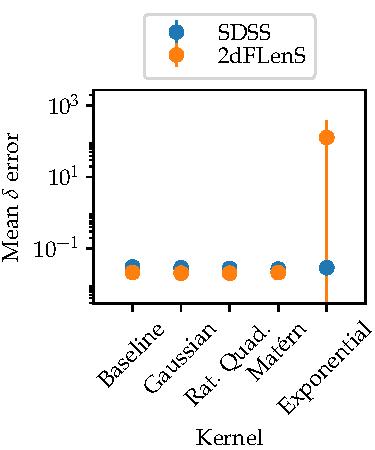
\includegraphics[width=0.4\textwidth]{linreg_kernelised_regularised.pdf}
    \caption{Error of regularised kernelised linear regression. The regularisation constant $\lambda$ is $0.001$.}
    \label{fig:linreg_kernelised_regularised}
  \end{wrapfigure}

We often wish to ensure that $\hat f$ relatively simple to prevent overfitting. We can make the assumption that every element of the weights vector $\bw$ is likely to be close to zero: \[
    p(w_i) = \cN(w_i \mid 0, \omega^2)
\] for some variance $\omega^2 > 0$.

We can then change the likelihood in \cref{eq:linearlikelihood} to account for this: \begin{align*}
    p\left(\hat f \;\middle|\; \cD\right) &= \prod_{i = 1}^{n} \cN\left(\hat y_i \;\middle|\; y_i, \sigma^2\right) \label{eq:linearlikelihood} \prod_{i = 1}^{m}\cN(w_i \mid 0, \omega^2) \\
    &= \prod_{i = 1}^{n} \frac{1}{\sqrt{2\pi\sigma^2}} \exp\left(-\frac{\left(\hat y_i - y_i\right)^2}{2\sigma^2}\right) \prod_{i = 1}^{m}\frac{1}{\sqrt{2\pi\omega^2}} \exp\left(-\frac{w_i^2}{2\omega^2}\right) \text{.}
\end{align*} Computing the negative log likelihood,\[
    -\log p\left(\hat f \;\middle|\; \cD\right) = \frac{n}{2}\log\left(2\pi\sigma^2\right) + \frac{1}{2\sigma^2}\sum_{i=1}^{n}\left(\hat y_i - y_i\right)^2 + \frac{m}{2}\log\left(2\pi\omega^2\right) + \frac{1}{2\omega^2}\sum_{i=1}^{m}w_i^2 \text{.}
\] Eliminating the constant terms and defining $\lambda \coloneqq \sigma^2 / \omega^2$, we find that \begin{align*}
    \argmin_{\bw} \left[- \log p\left(\hat f \;\middle|\; \cD\right)\right] &= \argmin_{\bw} \left(\frac{1}{2\sigma^2}\sum_{i=1}^{n}\left(\hat y_i - y_i\right)^2 + \frac{1}{2\omega^2}\sum_{i=1}^{m}w_i^2\right) \\
     &= \argmin_{\bw} \left(\frac12\sum
    _{i=1}^{n}\left(\hat y_i - y_i\right)^2 + \frac{\lambda}{2}\sum_{i=1}^{m}w_i^2\right) \\
    &= \argmin_{\bw} \left(\frac12\left(\hat \by - \by\right)^\top\left(\hat \by - \by\right) + \frac{\lambda}{2}\bw^\top\bw\right) \\
    &= \argmin_{\bw} \left(\frac12\left(\Phi \bw - \by\right)^\top\left(\Phi \bw - \by\right) + \frac{\lambda}{2}\bw^\top\bw\right) \text.
\end{align*}

Our loss now depends on $\bw$ and $\lambda$ and is given by \[
    E(\bw, \lambda) = \frac12\left(\Phi \bw - \by\right)^\top\left(\Phi \bw - \by\right) + \frac{\lambda}{2}\bw^\top\bw \text{,}
\] where $\lambda$ is our \textit{regularisation constant}: a higher value implies a simpler model, reducing the likelihood of overfitting, but increasing the chance of underfitting.

We can find $\bw$ that minimises the loss. Taking the derivative and setting it to $\mathbf{0}$,\[
    \frac{dE(\bw, \lambda)}{d\bw} = \Phi^\top(\Phi\bw - \by) + \lambda \bw = \mathbf{0} \text{.}
\] Solving,\[
    \bw = \left(\Phi^\top\Phi + \lambda I\right)^{-1}\Phi^\top\by \text.
\]

\section{Finding hyperparameters}

\jn{introduce}

  \subsection{Grid search}

  Grid search is one technique that permits us to find hyperparameters. We must first define a finite set of candidate hyperparameter configurations $H$.

  \jn{rewrite in algorithm2e}
  The algorithm is as follows:
  \begin{minted}[
    gobble=4,
    linenos,
    fontsize=\small,
    frame=lines,
    python3=true
  ]{python}
    def cross_validate(H, train_X, train_y, validation_X, validation_y)
        best_parameters = None
        best_score = float('-inf')

        for h in H:
            regressor.set_params(**h)
            regressor.train(train_X, train_y)
            score = regressor.score(validation_X, validation_y)

            if score > best_score:
                best_parameters = h

        return best_parameters
  \end{minted}

  The name \emph{grid search} comes from $H$ often being a Cartesian product of the options for each hyperparameter, forming a multidimensional `grid'.

  \subsection{Bayesian optimisation}
  Our regression has six hyperparameters: a length scale $\sigma_i$ for each of the five features and a regularisation constant $\lambda$. The high dimensionality of the hyperparameter space makes it difficult to find the optimal parameters using grid search. Bayesian optimisation may be used instead to speed up this process.

\jn{derive bayesian optimisation}

\subsection{Automatic relevance determination}
  \begin{figure}
    \centering
    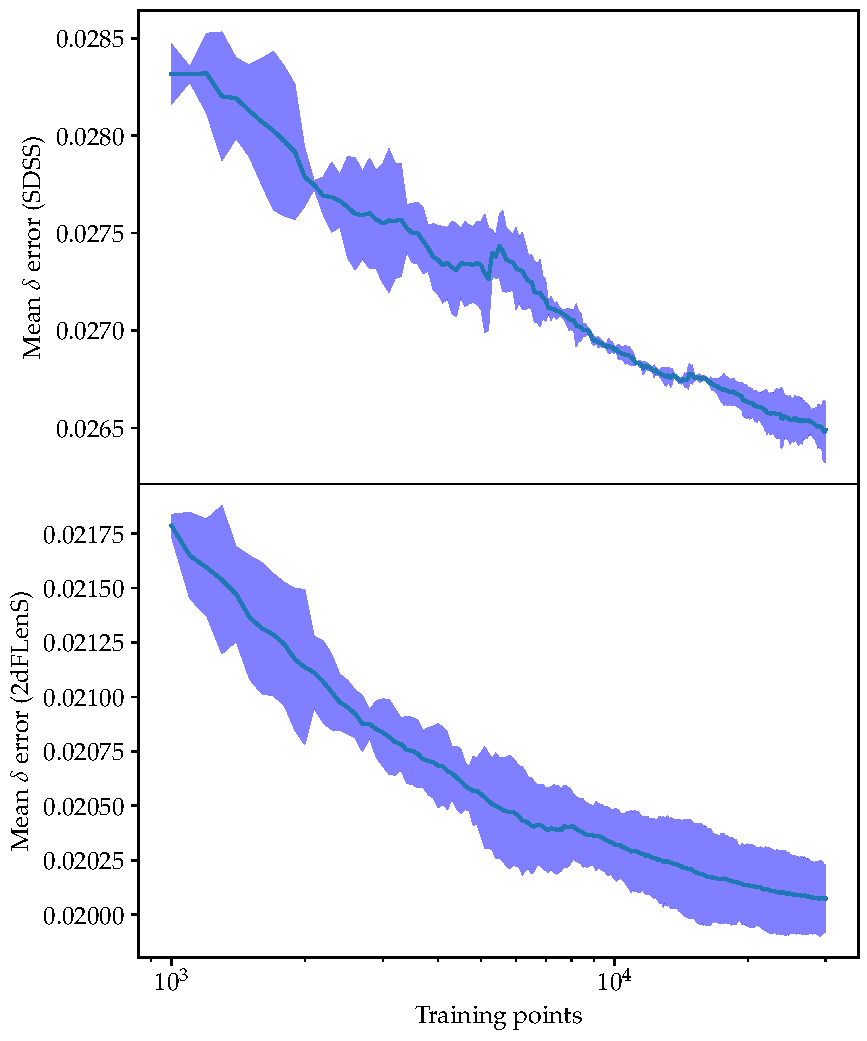
\includegraphics[width=0.9\textwidth]{passive_delta.pdf}
    \caption{Passive learning curve: Mean $\delta$ error plotted against the number of training points for both SDSS and 2dFLenS. The training points are chosen at random. The shaded interval represents the two-sigma confidence interval.}
    \label{fig:passive_delta}
  \end{figure}

  \begin{figure}
    \centering
    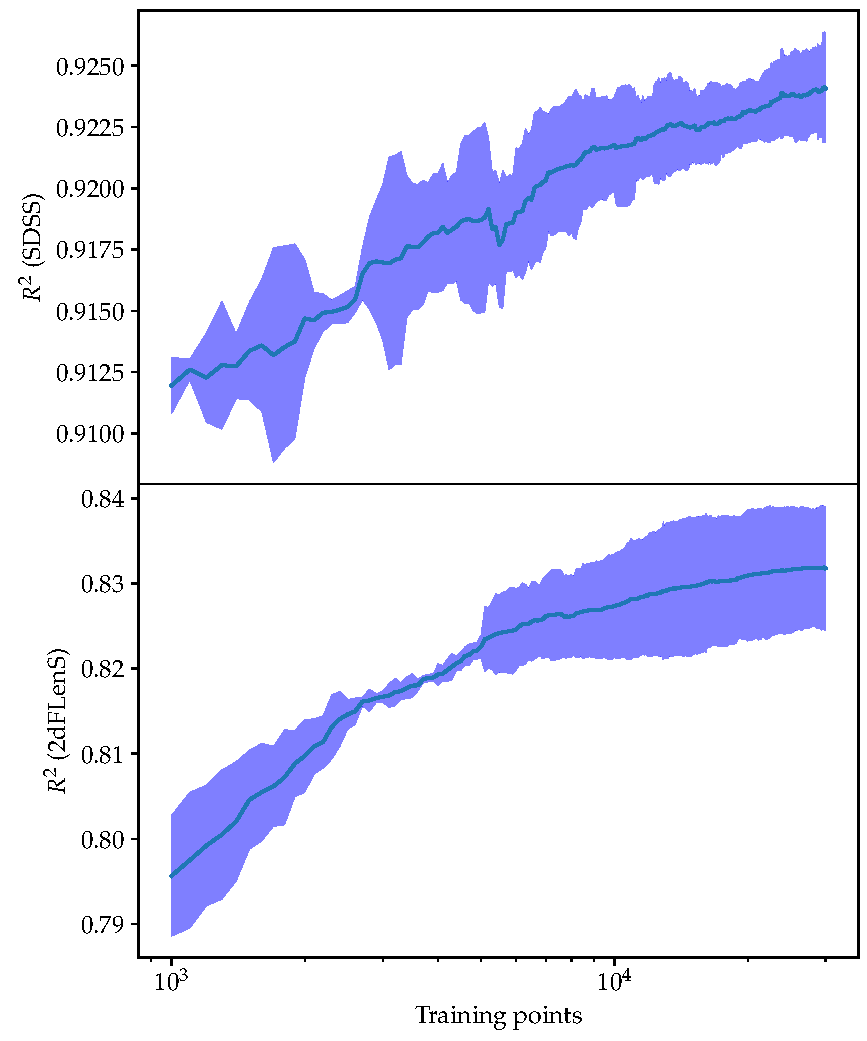
\includegraphics[width=0.9\textwidth]{passive_r2.pdf}
    \caption{Passive learning curve: $R^2$ error plotted against the number of training points for both SDSS and 2dFLenS. The training points are chosen at random. The shaded interval represents the two-sigma confidence interval.}
    \label{fig:passive_r2}
  \end{figure}

Automatic relevance determination (ARD) is another technique that may be used to find the hyperparameters for our Gaussian Process Regression.

Consider the problem of linear regression. We have a five-dimensional feature space $\cX$. The features have \jn{noise vairances?} variances $\lambda_1, \dots, \lambda_5$, respectively. We place a prior on our regression weights.

Our prior variance for each weight is proportional to the variance of the weight. We also assume that the weights are uncorrelated. Hence, our sum-of-squares loss function becomes \jn{how?}\[
    \frac12\norm{X\bw - \by}^2 + \alpha \bw^\top \Lambda \bw \text.
\]

\jn{now talk about that weird convergence bullshit for the regularisation constant}

\jn{we don't care about pruning right? because we're not pruning...}

\section{Gaussian process regression}
\jn{rewrite this sanely}

Gaussian process regression (GPR) is a predictor that yields confidence intervals for its own predictions. This is very useful when performing active learning. We derive GPR here.

A Gaussian process is a distribution over functions. Formally, a Gaussian process is defined as a `collection of random variables, any finite number of which have a joint Gaussian distribution.'\citep{GPBook}

Defining \begin{align*}
    m(\vec{x}) &\coloneqq \bbE[f(\vec{x})] \text, \\
    k(\vec{x}, \vec{x}') &\coloneqq \bbE[(f(\vec{x}) - m(\vec{x}))(f(\vec{x'}) - m(\vec{x'}))],
\end{align*} we write \[
    f(\vec{x}) \sim \cG\cP(m(\vec{x}), k(\vec{x}, \vec{x'}))\text.
\]

We write \begin{align*}
    \vec y &\coloneqq (y_1, \dots, y_n)^\intercal \text, \\
    X &\coloneqq (\vec{x_1}, \dots, \vec{x_n})^\intercal \text, \\
    K(X, X) &\coloneqq \begin{bmatrix}
        k(\vec{x_1}, \vec{x_1}) & \cdots & k(\vec{x_1}, \vec{x_n}) \\
        \vdots & \ddots & \vdots \\
        k(\vec{x_n}, \vec{x_1}) & \cdots & k(\vec{x_n}, \vec{x_n})
    \end{bmatrix}\text.
\end{align*}

Then $\cov(\vec{y}) = K(X, X) + \sigma_n^2I$.

Let $\vec{f_*}$ be the test predictions and $X_*$ be the test inputs. Under the prior, we have that the joint distribution of the observed targets and of the function values at the test locations is \[
    \begin{bmatrix}
        \vec{y} \\ \vec{f_*}
    \end{bmatrix} \sim \cN\left(\vec0, \begin{bmatrix}
        K(X, X) + \sigma_n^2I & K(X, X_*) \\
        K(X_*, X) & K(X_*, X_*)
    \end{bmatrix}\right)\text.
\]

It can then be derived that \[
    \vec{f_*} \mid X, \vec{y}, X_* \sim \cN\left(\overline{\vec{f_*}}, \cov(\vec{f_*})\right)\text,
\] where \[
    \overline{\vec{f_*}} = K(X_*, X)[K(X, X) + \sigma_n^2I]^{-1}\vec{y}\text,
\] and \[
    \cov(\vec{f_*}) = K(X_*, X_*) - K(X_*, X)[K(X, X) + \sigma_n^2I]^{-1}K(X, X_*)\text.
\]

The value for $\vec{f_*}$ that has the highest probability is the mean of the Gaussian from which it is sampled. Hence, we can predict that \begin{equation}
    \label{eq:pred}
    \vec{f_*} \approx K(X_*, X)[K(X, X) + \sigma_n^2I]^{-1}\vec{y}\text,
\end{equation} with the variance for each element of the vector being\[
    \var(\vec{f_*}_i) = \left( K(X_*, X_*) - K(X_*, X)[K(X, X) + \sigma_n^2I]^{-1}K(X, X_*) \right)_{ii}\text.
\]

One can observe from \cref{eq:pred} that the prediction is a linear combination of the observations $\vec{y}$. This is in contrast to linear regression, where the prediction is a linear combination of the inputs.

\subsection{Equivalence to kernelised linear regression}

Observe that \cref{eq:pred} is the equation for kernelised linear regression with regularisation, where $\lambda=\sigma_n^2$. Thus, Gaussian Process regression and kernelised regular regression always return the same expected value, although kernelised linear regression is unable to estimate the variance of that prediction.

\section{Approximating Gaussian processes}

Gaussian process regression relies on our calculation of $(K+\sigma_n^2)^{-1}$. This has a large time complexity\footnote{$O(n^3)$ for a naive implementation; $O(n^{2.373})$ for an optimised method based on the Coppersmith–Winograd algorithm.\jn{reference}}. This does not scale well to large training sets. Instead, we can approximate GPR with algorithms of a lower time complexity.

\subsection{Low-rank approximation}

We can approximate this matrix product with a complexity that is linear in $n$. We can do so by approximating the kernel with a finitely-dimensional set of features, and reversing the kernelisation.

Let $\Phi \in \bbR^{n \times d'}$ for $d' \ll n$ be our kernel approximation for the training set, letting $K \approx \Phi \Phi^\top$. Let $\bphi \in \bbR^{d'}$ be the kernel approximation for the value we wish to predict for, so $K_* \approx \Phi \bphi$. We have that,\begin{align*}
    K_*^\top(K+\sigma_n^2)^{-1} &\approx \bphi^\top\Phi^\top  \left(\Phi \Phi^\top + \sigma_n^2I\right)^{-1} \\
    &= \bphi^\top\Phi^\top  \left( \sigma_n^{-2}I - \sigma_n^{-2}\Phi(\sigma_n^{2} + \Phi^\top\Phi)^{-1}\Phi^\top\right) \\
    &=  \sigma_n^{-2}\bphi^\top\Phi^\top - \sigma_n^{-2}\bphi^\top\Phi^\top \Phi(\sigma_n^{2} + \Phi^\top\Phi)^{-1}\Phi^\top \text{,}
\end{align*} where we apply the Woodbury matrix identity to reduce the rank of the matrix being inverted.

Substituting \jn{blah} into \jn{blah} and \jn{blah}, \[
    \hat f(\bx) = \sigma_n^{-2} \bphi^\top\Phi^\top\by - \sigma_n^{-2} \bphi^\top\Phi^\top\Phi(\sigma_n^{2} + \Phi^\top\Phi)^{-1}\Phi^\top\by
\] and \[
    \var \hat f(\bx) = \bphi^\top\bphi - \sigma_n^{-2}\Phi^\top \bphi^\top\bphi\Phi - \sigma_n^{-2}\Phi^\top \bphi^\top\Phi(\sigma_n^{2} + \Phi^\top\Phi)^{-1}\Phi^\top\bphi\Phi\text.
\]Since the size of the matrix being inverted no longer depends on $n$, this is a linear-time approximation.

Numerical instabilities present difficulties for small $\sigma_n^2$ as the matrix $(\Phi\Phi^\top + \sigma_n^2I)$ becomes closer to being singular.

\subsection{Linear regression and KDE}

\jn{make this sane}

The mean of Gaussian Process Regression can also be approximated by linear regression. Letting $\Phi$ be the kernel approximation on the training set, we find that the regression weights are\[
    \bw = \left(\Phi^\top\Phi + \sigma_n^2 I\right) \Phi^\top\by\text,
\] where $\sigma_n^2$ becomes the regularisation constant. This can be computed in $O(nf)$ time by solving the linear equation instead of directly performing the matrix inversion.

It remains to find an approximation to the variance predicted by Gaussian Process regression. Kernel density estimation can be used to approximate this. Let $D$ be the density estimator. Then we expect $\left(D(\bx)\right)^1$ and $\var f(\bx)$ to have a monotonic relationship.

The actual relationship could probably be found by regression on the estimated densities and the estimated variances of an artificially generated dataset.

This method is less prone to numerical instabilities than my favourite approximation. However it was not used in this work, as a more direct approximation was available.


\chapter{Active learning}

In regression on photometric redshifts, it is expensive to obtain new labels for training samples: a telescope can only measure the spectrum of one galaxy at a time. However, photometric data is cheap, so we have a large pool of unlabelled objects. We wish to spend our telescope time labelling the objects that are the most likely to improve the accuracy of our model. Active learning is a technique that permits this.

In active learning, we selectively find labels to samples based on their potential for improving our model. \jn{CITE} Given an existing model and a pool of unlabelled samples, a \textit{recommender} chooses samples based on its policy. It is only after a sample is recommended that we query its label and add it to our model's training set. A procedure is presented in \cref{alg:active-learning}.

A recommendation strategy is effective if its choices yield a more accurate model than a randomly selected training set. Active learning then reduces, compared to the naïve approach, the number of labelled samples needed to achieve a predictor of a desired accuracy, saving resources.

\begin{algorithm}[t]
    \KwData{
      \\\quad A recommender $\pi : \cP(\cX) \times \bbN \to \cP(\cX)$,
      \\\quad A function $\hat F : \cP(\cX \times \cY) \to \cF$ generating a predictor from training samples,
      \\\quad A training sample pool $P \subseteq \cX$,
      \\\quad A labeller $\tilde f : P \to \cY$,
      \\\quad Step size $t \in \bbZ_{>0}$,
      \\\quad An error function $e \in \mathcal{E}$,
      \\\quad A desired maximum error $\mathrm{err}_\mathrm{max}$.
    }
    \KwResult{A predictor $\hat f : \cX \to \cY$ with $e(\hat f) \leq e_\mathrm{\max}$ or error}

    \lIf*{$\abs{P} < t$}{\Return error}

    $\cD_{\cX} \gets t$ samples drawn randomly from $P$ without replacement

    $P \gets P \setminus \cD_{\cX}$ \hfill (remove chosen samples from pool)

    $\cD \gets \left\{\left(\bx, \tilde f(\bx)\right) \;\middle|\; \bx \in \cD_{\cX} \right\}$ \hfill (label chosen samples)

    $\hat f \gets F(\cD)$ \hfill (train model)

    $\mathrm{err} \gets e\left(\hat f\right)$ \hfill (compute error)

    \While{$\mathrm{err} > \mathrm{err}_\mathrm{max}$}{
      \lIf*{$\abs{P} < t$}{\Return error}

      $\cD_{\cX} \gets \pi(P, t)$ \hfill (get recommendations)

      $P \gets P \setminus \cD_{\cX}$ \hfill (remove chosen samples from pool)

      $\cD \gets \cD \cup \left\{\left(\bx, \tilde f(\bx)\right) \;\middle|\; \bx \in \cD_{\cX} \right\}$ \hfill (label chosen samples)

      $\hat f \gets F(\cD)$ \hfill (train model on all samples)

      $\mathrm{err} \gets e\left(\hat f\right)$ \hfill (compute error)
    }

    \Return $\hat f$

    \caption{The active learning procedure.}
    \label{alg:active-learning}
\end{algorithm}

\section{Benefits}

\jn{TODO: Write this section, time permitting. Back up with statistics. If out of time, delete it.}

\section{Recommenders}

In active learning, a \textit{recommender} is a function\footnote{To be precise, a recommender is not always a function as it is permitted to be nondeterministic.} that predicts \jn{estimates?} what samples are the most useful to label. \jn{CITE} It can be thought of in two equivalent ways.

A recommender can be thought of as a function $\pi : \cP(\cX) \times \bbN \to \cP(\cX)$, where $\pi(P, r)$ returns the $r$ most preferred samples from the sample pool $P$. A recommender can also be a function $\varpi : \cX \to \bbR$. Then $\varpi(\bx)$ returns the preference score it assigns to $\bx$, with higher scores being preferred. Define $\Pi$ to be the space of all recommenders.

Given a recommender $\varpi$ returning a score, we can define a recommender $\pi$ returning a set of samples. One way to obtain $\pi(P, r)$ is by choosing the top $r$ samples from $P$ as scored by $\varpi$.

Similarly, given a recommender $\pi$ returing a set of samples, we can define a recommender $\varpi$ returning a score. Assuming a fixed pool $P \in \cP(\cX)$, for all $\bx\in\cX$, define\[
  \varpi(\bx) \coloneqq -\min \{ i = 1, \dots, \abs{P} \mid \bx \in \pi(\cX, i)\} \text.
\] Then the score $\varpi$ assigns to $\bx$ is the negation of its preference index in $\pi$.


\section{Relation to Bayesian optimisation with Gaussian processes}

\jn{TODO: Write this section, time permitting. Else, delete it.}


\section{Measuring performance}

\subsection{Learning curves}
A learning curve tracks the performance of a model with a given recommender. \jn{CITE} Let $T = \{t_1, \dots, t_r\} \subset \bbN$ with $t_1 < \dots < t_r$ be the counts of training points that we try. Then the learning curve is a function $\ell : T \to \bbR_{\geq0}$, whose output is an error.

For a recommender $\pi$ and a model $F : \cP(\cX \times \cY) \to \hat\cF$, we generate the learning curve $\ell$ with \cref{alg:generate-learning-curve}. Intuitively, we begin by training $F$ with $t_1$ random samples and measuring its performance. We then repeatedly add points recommended by $\pi$, train the model, and measure its performance. This gives us $F$'s performance as a function of the cardinality of the training.

We can qualitatively describe the performance of a recommender by examining the learning curve it generates. In general, the better the accuracy of $F$ trained on points given by $\pi$, the better $\pi$ is.

An example of a learning curve can be seen in \cref{fig:uncertainty_dz1}. In that figure, the uncertainty recommender clearly outperforms the passive (random) recommender.

\begin{algorithm}[t]
    \KwData{
      \\\quad A recommender $\pi : \cP(\cX) \times \bbN \to \cP(\cX)$,
      \\\quad A function $F : \cP(\cX \times \cY) \to \hat\cF$ generating a predictor from training samples,
      \\\quad A function $e : \hat\cF \to \bbR_{\geq0}$ yielding the error of a predictor,
      \\\quad A training sample pool $P \subseteq \cX$,
      \\\quad Labels for samples in $P$,
      \\\quad Training example counts to try $T = \{t_1, \dots, t_r\} \subset \bbN$ with $t_1 < \dots < t_r$.
    }
    \KwResult{A learning curve $\ell : T \to \bbR_{\geq0}$.}

    $\cD_\cX \gets t_1$ samples drawn randomly from $P$ without replcement

    $P \gets P \setminus \cD_\cX$ \hfill (remove chosen samples from pool)

    $\cD \gets \left\{ \left(\bx, \tilde f(\bx)\right) \;\middle|\; \bx \in \cD_\cX \right\}$ \hfill (label chosen samples)

    $\hat f \gets F(\cD)$ \hfill (train model)

    $\ell(t_1) \gets e\left(\hat f\right)$ \hfill (compute error)

    \For{$i \in 2, \dots, r$}{
      $\cD_\cX \gets \pi(P, t_i)$ \hfill (get recommendations)

      $P \gets P \setminus \cD_\cX$ \hfill (remove chosen samples from pool)

      $\cD \gets \cD \cup \left\{\left(\bx, \tilde f(\bx)\right)\;\middle|\;\bx \in \cD_\cX\right\}$ \hfill (label chosen samples)

      $\hat f \gets F(\cD)$ \hfill (train model)

      $\ell(t_i) \gets e\left(\hat f\right)$ \hfill (compute error)
    }

    \Return $\ell$
    \caption{Generating a learning curve.}
    \label{alg:generate-learning-curve}
\end{algorithm}

\subsection{Deficiency}

\begin{wrapfigure}{R}{0.5\textwidth}
    \centering
    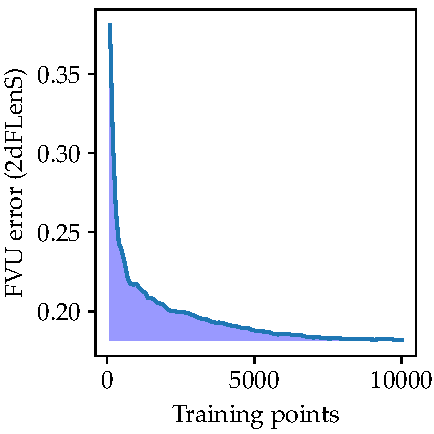
\includegraphics[width=0.5\textwidth]{deficiency_example.pdf}
    \caption{A passive learning curve for 2dFLenS. Its deficiency is the area of the shaded region, in this case 135.7.}
    \label{fig:deficiency_example}
  \end{wrapfigure}

The deficiency $d$ is a function $d : \fD \times \fF \times \cE \times \cT \times \Pi \to \bbR$. Intuitively, $d(P, F, e, T, \pi)$ measures the room for improvement that a recommender $\pi \in \Pi$ has on a model $F \in \fF$, a training set pool $P \in \fD$, at times $T \in \cT$, according to an error function $e \in \cE$. In general, the lower the deficiency, the better $\pi$ performs on our predictor and dataset. \jn{CITE}

To define $d(P, F, e, T, \pi)$, let $\ell : T \to \bbR_{\geq0}$ be the learning curve with a predictor $F$, a recommender $\pi$, a candidate pool $P$, and an error function $e$ and $F$ at times $T = \{t_1, \dots, t_r\}$ ordered in ascending order. Generally, $\ell$ reach its minimum at $t_r$. This is because, in general, models perform better with more training samples; hence, training on all available samples is likely to yield the best possible model. We use $\ell(t_r)$ as a baseline for a `perfect' recommender.\footnote{We use the word `perfect' rather loosely, as it is impossble to define a truly perfect recommender. In most cases, even the best possible recommender will not reach a deficiency of $0$ as no proper subset of $P$ will yield comparable performance to the entirety of $P$.}

Then we define $d$ to be the signed area between $\ell$ and the line $y = \ell(t_r)$, as shown in \cref{fig:deficiency_example}. Since $\ell$ is sampled at discrete intervals, we compute it by applying the trapezoidal rule: \[
  d(\pi; P, F, e, T) = \sum_{i=1}^{r-1} \frac{t_{i+1} - t_i}{2}\Big(\big[\ell(t_i) - \ell(t_r)\big] + \big[\ell(t_i) - \ell(t_r)\big]\Big) \text.
\]

Observe that the deficiency is permitted to be negative. This may occur if $F$ trained on a subset of $P$ with size $t_i < t_r$ performs better than $F$ trained on the entirety of $P$. Then $\ell(t_i) - \ell(t_r)$ is negative, so the integral is permitted to be negative. This occurs very rarely as most models benefit from larger training sets.

For a fixed, $P$, $F$, $e$, and $T$, we may compute the deficiencies of recommenders $\pi$ and $\pi'$ to compare them. Let $\ell$ and $\ell'$ be the learning curves of $\pi$ and $\pi'$ respectively. Then $\ell(t_r) = \ell'(t_r)$, since $F$ is always trained on the entire pool $P$ at $t_r$.\footnote{Whilst this is true mathematically, in reality $\ell(t_r)$ and $\ell'(t_r)$ are approximately but not exactly equal due to numerical inaccuracies. To permit the deficiencies to be compared directly, we find the average of the individual baselines and use it to compute the deficiencies.} Then $d(\pi)$ is the area between $\ell$ and a baseline, and $d(\pi')$ is the area between $\ell$ and the same baseline. Since the baseline is the identcal, it is possible to directly compare the deficiencies to rank the recommenders.

\section{Possible recommenders}

\subsection{Recommenders for classification}

\jn{TODO: Time permitting, provide background on recommenders available for active learning on classification. Else, delete this subsection.}

\subsection{Passive}

The passive recommender is the baseline upon which we wish to improve. It yields random samples from the candidate pool. \jn{CITE} This makes it equivalent to adding extra training points without utilising any active learning techniques. The passive learning curves we use as a baseline are shown in \cref{fig:passive_dz}, \cref{fig:passive_fvu}, and \cref{fig:passive_sdss}. We use these to assess the performance of our active learning techniques.

\subsection{Uncertainty}
  \begin{figure}
    \centering
    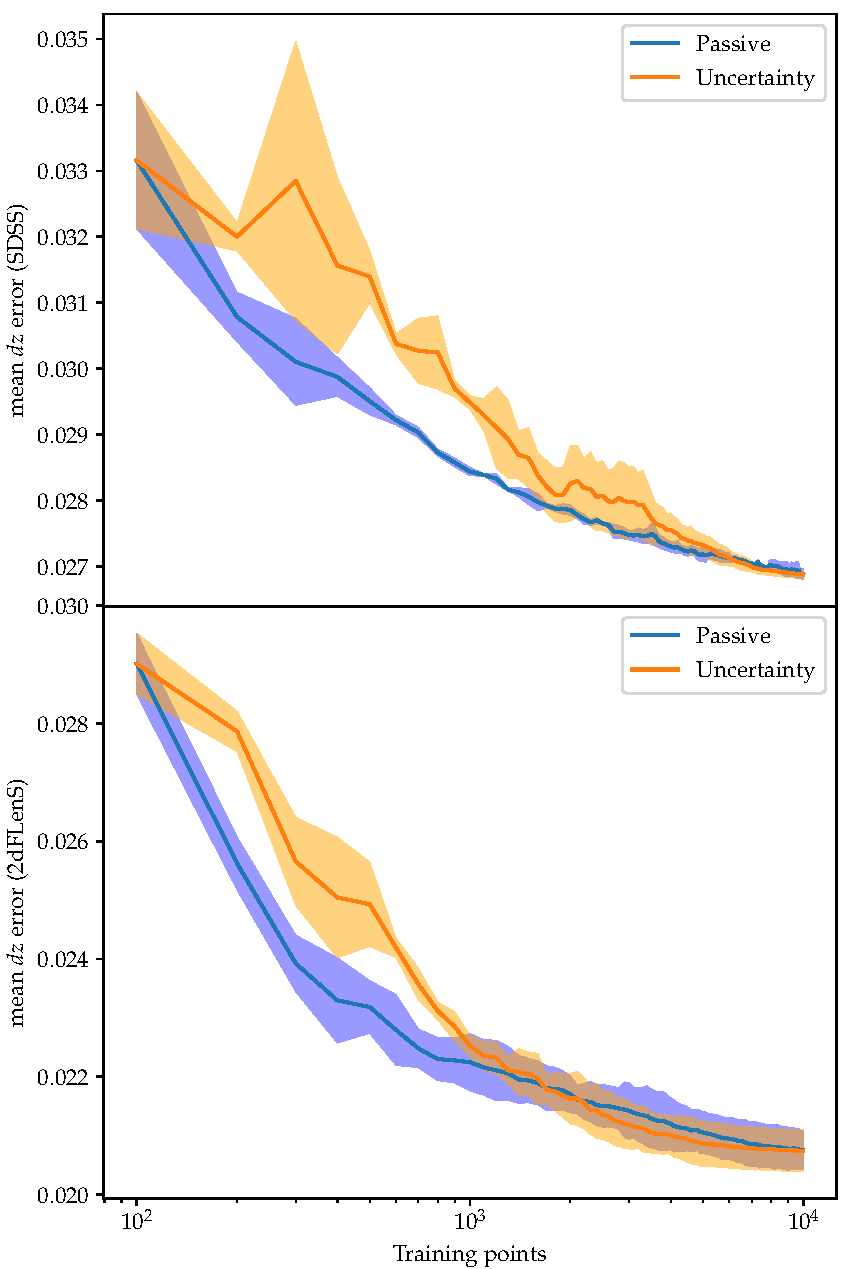
\includegraphics[width=0.9\textwidth]{uncertainty_dz1.pdf}
    \caption{Learning curve: mean $dz$ error plotted against the number of training points for both SDSS and 2dFLenS. The training points are chosen either at random (Passive) or using uncertainty recommendation with a step size of $100$. The shaded interval represents the one-sigma confidence interval.}
    \label{fig:uncertainty_dz1}
  \end{figure}

  \begin{figure}
    \centering
    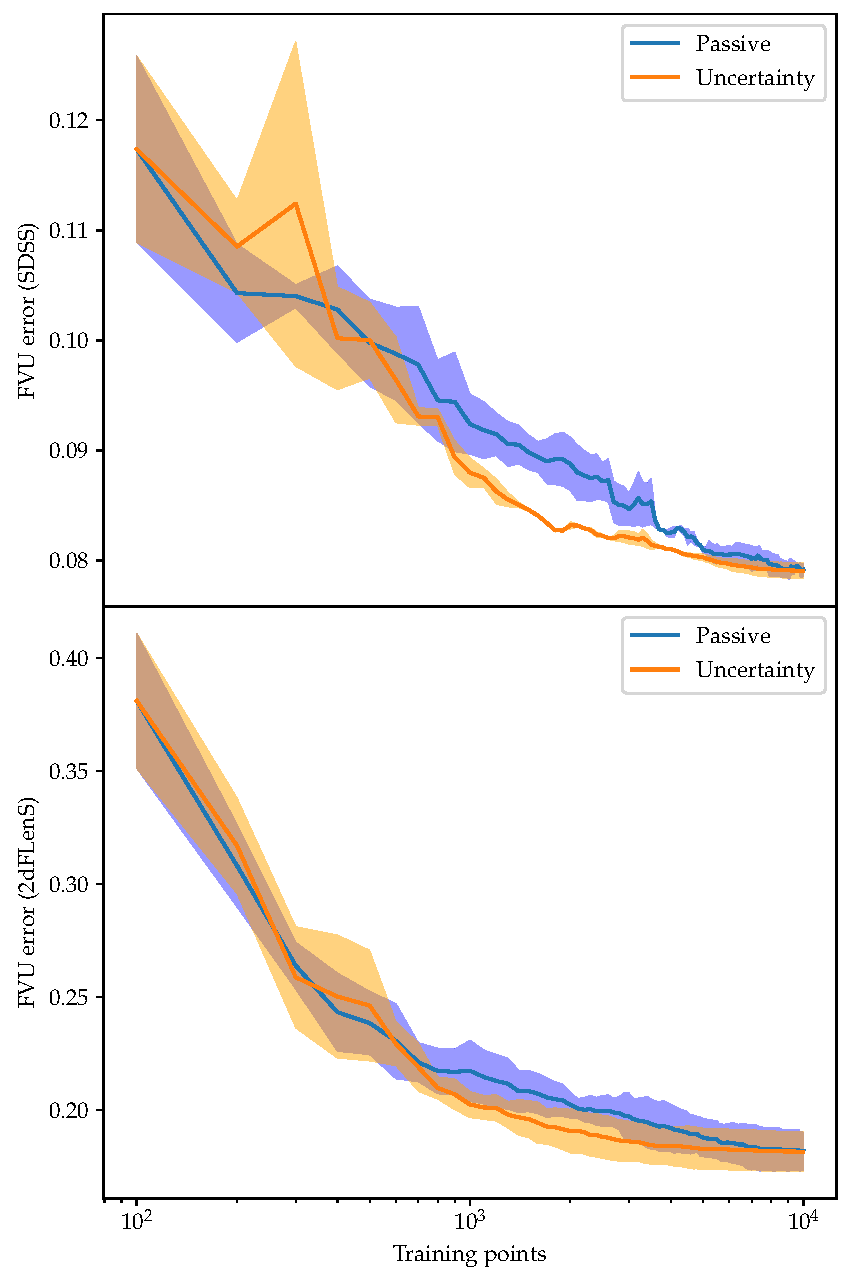
\includegraphics[width=0.9\textwidth]{uncertainty_fvu1.pdf}
    \caption{Learning curve: FVU error plotted against the number of training points for both SDSS and 2dFLenS. The training points are chosen either at random (Passive) or using uncertainty recommendation with a step size of $100$. The shaded interval represents the one-sigma confidence interval.}
    \label{fig:uncertainty_fvu1}
  \end{figure}

Let $\var\hat f : \cX \to \bbR_{\geq0}$ be the variance returned by Gaussian process regression. The uncertainty recommender is defined as a function $\varphi : \cX \to \bbR$ such that \[
    \varphi(\bx) = \var\hat f(\bx) \text.
\]

Intuitively, it returns the points that we are the most uncertain about. If we are uncertain about a point, then we have less information about that particular area of the feature space. Hence the points that we are uncertain about would be good additions to the training set.

Learning curves for SDSS and 2dFLenS with the mean $dz$ error are shown in \cref{fig:uncertainty_dz1}. Learning curves for the FVU error are shown in \cref{fig:uncertainty_fvu1}. We see that whereas uncertainty recommendation performs well in the later stages of training, it works rather poorly at the start. This is because we end up focusing on points that we are very unsure about, which tend to be on the long tail of the distribution. Since, in our case, the distribution is five-dimensional, this is a very poor strategy, as we spread out our efforts and neglect the core of the distribution.

\subsection{Density}

  \begin{figure}
    \centering
    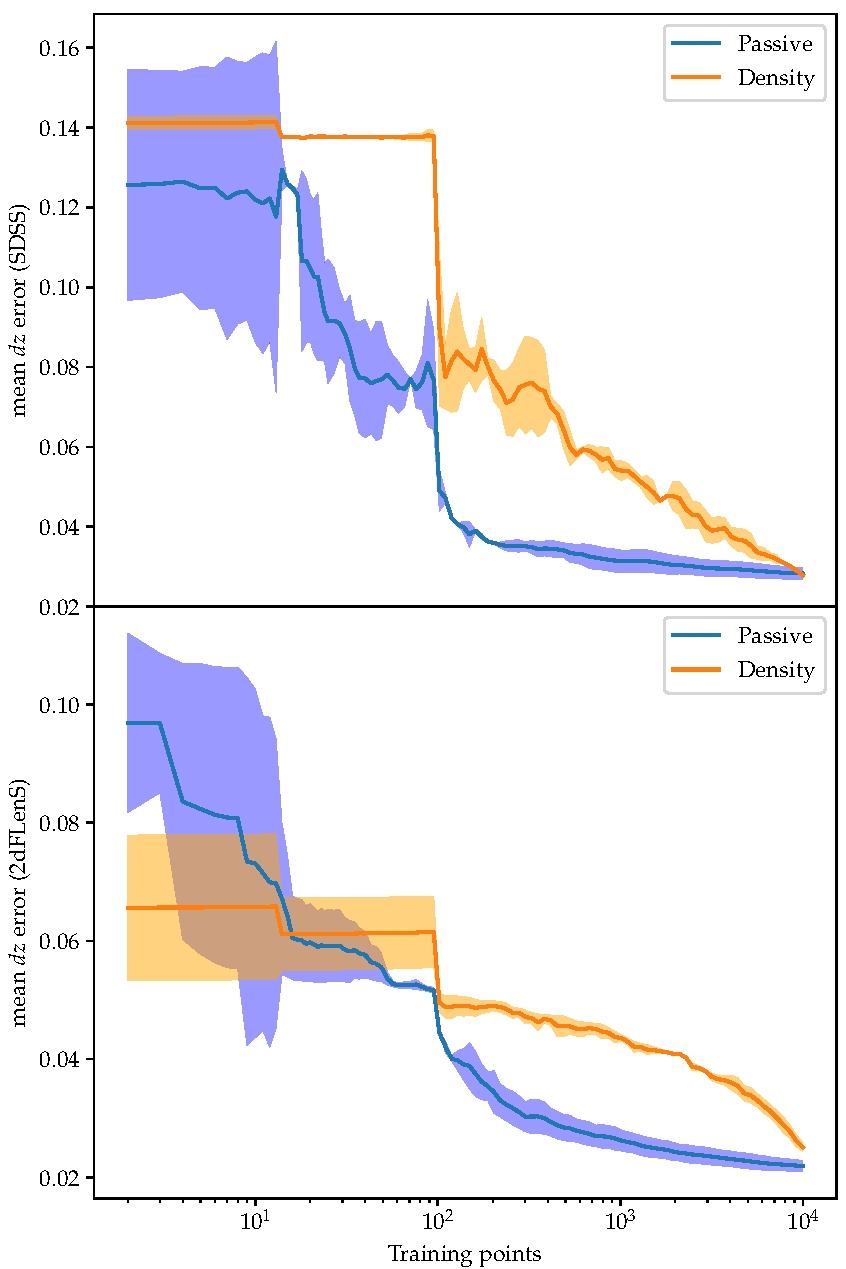
\includegraphics[width=0.9\textwidth]{density_dz1.pdf}
    \caption{Learning curve: mean $dz$ error plotted against the number of training points for both SDSS and 2dFLenS. The training points are chosen either at random (Passive) or using density recommendation with a logarithmic step size. Each curve begins with two data points chosen by its own recommender. ARD is used to find hyperparameters at $t=2$, $14$, and $100$. The density is approximated as a Gaussian. The shaded interval represents the one-sigma confidence interval.}
    \label{fig:density_dz1}
  \end{figure}

  \begin{figure}
    \centering
    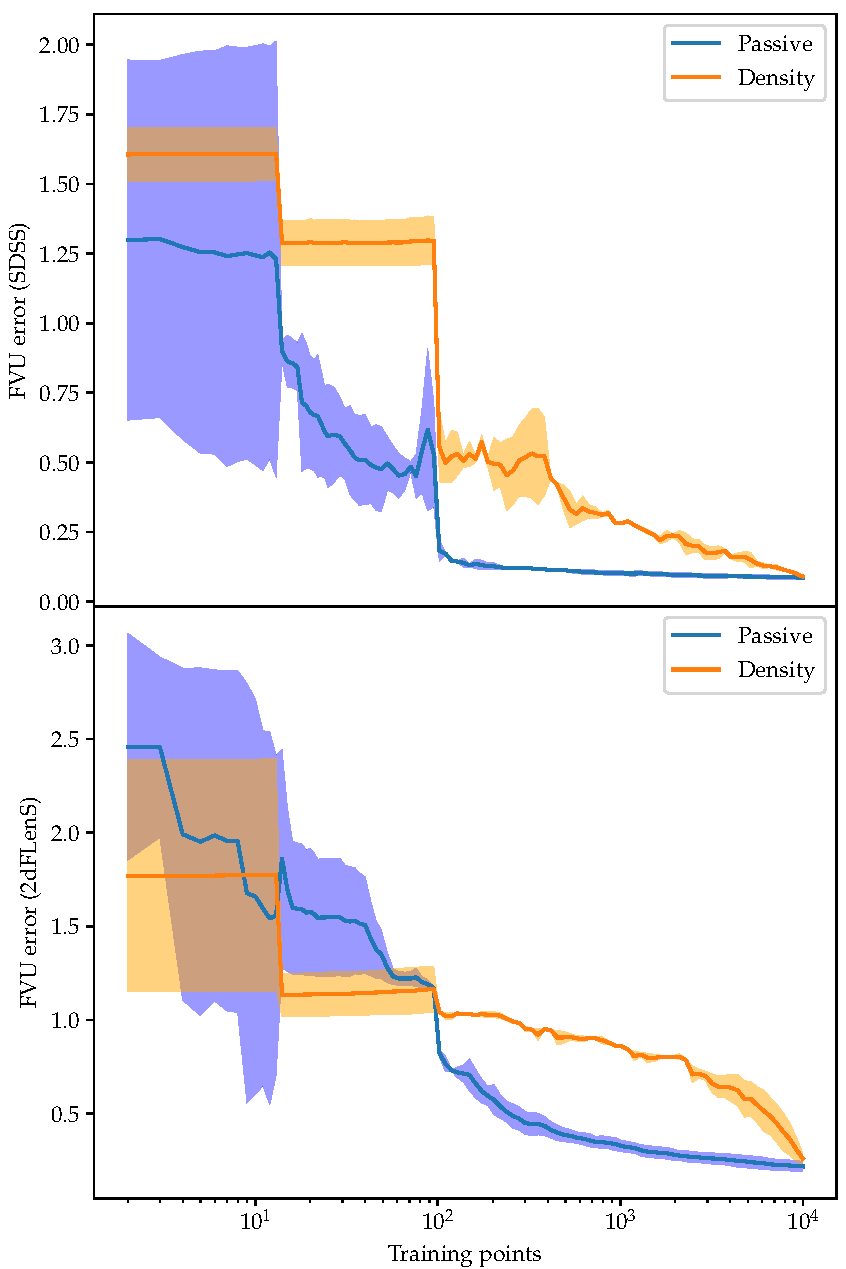
\includegraphics[width=0.9\textwidth]{density_fvu1.pdf}
    \caption{Learning curve: FVU error plotted against the number of training points for both SDSS and 2dFLenS. The training points are chosen either at random (Passive) or using density recommendation with a logarithmic step size. Each curve begins with two data points chosen by its own recommender. ARD is used to find hyperparameters at $t=2$, $14$, and $100$. The density is approximated as a Gaussian. The shaded interval represents the one-sigma confidence interval.}
    \label{fig:density_fvu1}
  \end{figure}{}

  Let $D : \cX \to \bbR^+$ be a density function for the dataset. The density estimator is a function $\varpi : \cX \to \bbR$ such that \[
    \varpi(\bx) \coloneqq D(x) \text.
  \]

  If we do not know the true distribution of the dataset, we can estimate it. Gaussian mixture models and kernel density estimation are two possible approaches. We use a simple Gaussian with the mean and covariance of our dataset.

  We plot the learning curves for SDSS and 2dFLenS under density recommendation and mean $dz$ error in \cref{fig:density_dz1}. Similar curves for the FVU error are shown in \cref{fig:density_fvu1}. We note that this recommendation strategy yields good results at the start of the learning curve, when we have trained on very few sampels. However, later on the curve flattens out and no longer produces very good results, being overtaken by uncertainty recommendation.

\subsection{Boltzmann sampling}

  \begin{figure}
    \centering
    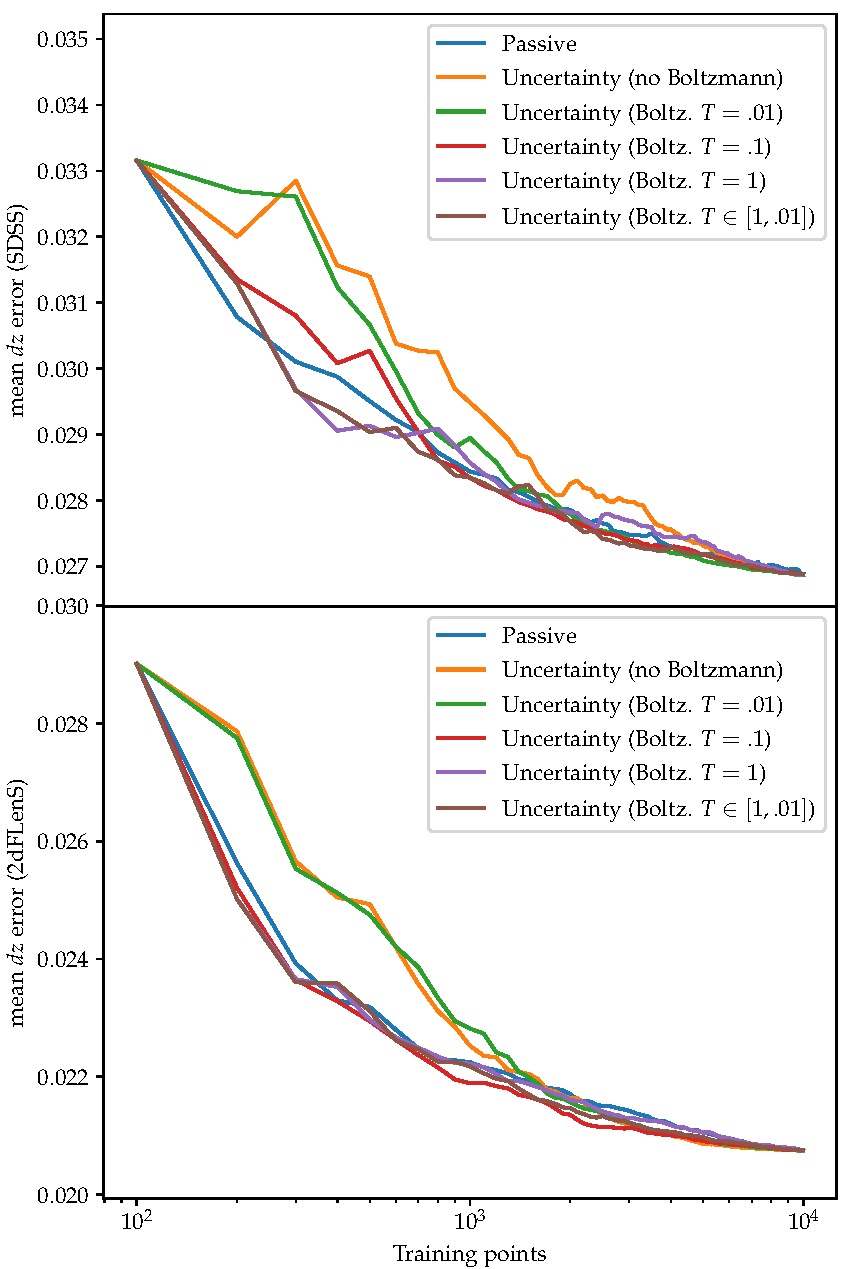
\includegraphics[width=0.9\textwidth]{boltz_uncertainty_dz1.pdf}
    \caption{Learning curve: mean $dz$ error plotted against the number of training points for both SDSS and 2dFLenS. The training points are chosen either at random (passive) or using uncertainty recommendation with a step size of $100$. Boltzmann sampling is applied to some curves, either with a constant temperature or a temperature logrithmically interpolated between two values.}
    \label{fig:boltz_uncertainty_dz1}
  \end{figure}

  \begin{figure}
    \centering
    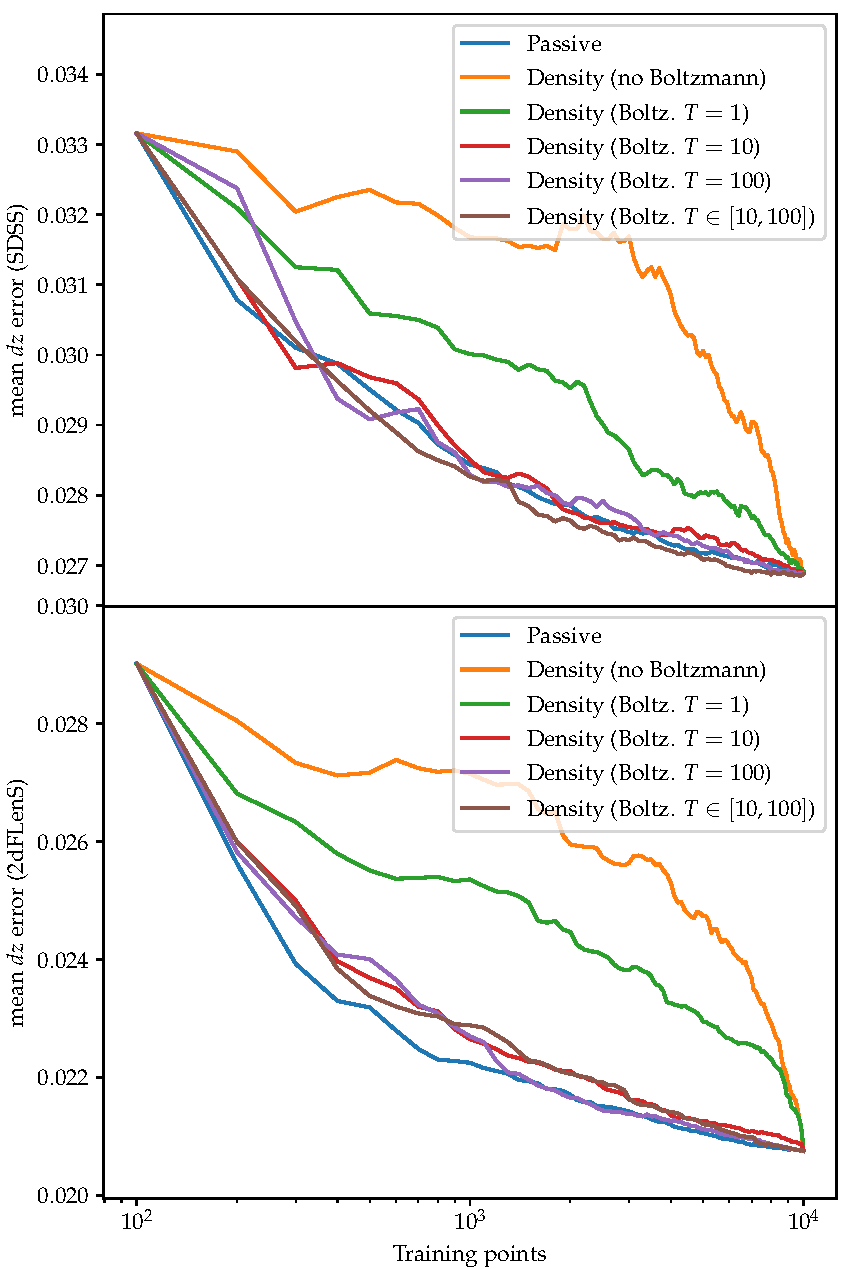
\includegraphics[width=0.9\textwidth]{boltz_density_dz1.pdf}
    \caption{Learning curve: mean $dz$ error plotted against the number of training points for both SDSS and 2dFLenS. The training points are chosen either at random (passive) or using density recommendation with a step size of $100$. Boltzmann sampling is applied to some curves, either with a constant temperature or a temperature logrithmically interpolated between two values.}
    \label{fig:boltz_density_dz1}
  \end{figure}

\begin{table}
\centering
\begin{subtable}{.5\textwidth}
\centering

\begin{tabular}{l | c c}
    & SDSS & 2dFLenS \\
    \hline
    Passive & 6.1 & 5.9 \\
    Uncert. (no Boltz.) & 8.7 & 6.2 \\
    Uncert. ($T = .01$) & 6.4 & 6.4 \\
    Uncert. ($T = .1$) & 5.7 & 4.4 \\
    Uncert. ($T = 1$) & 6.4 & 5.6 \\
    Uncert. ($T \in [1,.01]$) & 5.2 & 4.9 \\
    Density (no Boltz.) & 30 & 39 \\
    Density ($T = 1$) & 15 & 25 \\
    Density ($T = 10$) & 7.1 & 8.5 \\
    Density ($T = 100$) & 6.6 & 6.9 \\
    Density ($T \in [10,100]$) & 4.9 & 7.9 \\
\end{tabular}

\caption{Mean $dz$ error deficiencies}
\end{subtable}% <---- don't forget this %
\begin{subtable}{.5\textwidth}
\centering

\begin{tabular}{l | c c}
    & SDSS & 2dFLenS \\
    \hline
    Passive & 48 & 135 \\
    Uncert. (no Boltz.) & 31 & 86 \\
    Uncert. ($T = .01$) & 26 & 89 \\
    Uncert. ($T = .1$) & 24 & 64 \\
    Uncert. ($T = 1$) & 39 & 122 \\
    Uncert. ($T \in [1,.01]$) & 34 & 92 \\
    Density (no Boltz.) & 204 & 1196 \\
    Density ($T = 1$) & 124 & 838 \\
    Density ($T = 10$) & 47 & 243 \\
    Density ($T = 100$) & 36 & 178 \\
    Density ($T \in [10,100]$) & 43 & 238 \\
\end{tabular}

\caption{FVU error deficiencies}
\end{subtable}

\caption{Deficiency of passive, uncertainty, and density recommenders. Training took place with a step size of 100. Boltzmann sampling is applied to some recommenders, either with a constant temperature or a temperature logarithmically interpolated between the marked values.}
\label{table:boltzmann_deficiencies}
\end{table}


Consider a physical system that occupies one of $M$ possible states. Let $T > 0$ be the temperature of the system. For each $i=1, \dots, M$, the state $s_i$ has potential energy $\varepsilon_i$. If $\varepsilon_i < \varepsilon_{i'}$, then we must input energy equalling $\varepsilon_{i'} - \varepsilon_i$ to move from the state $s_i$ to $s_{i'}$. As an example, consider a hydrogen atom consisting of a nucleus and an electron. The electron occupies one of two shells around the nucleus: the inner shell or the outer shell. Energy is required to move this electron the inner shell to the outer shell; hence, the state of lying in the outer shell is of higher energy.

A system seeks to minimise its energy, resulting in a non-uniform probability of states. Higher-energy states are improbable but not impossible, particularly in high temperatures: a sufficiently hot gas will become ionised, entering a higher-energy state. The probability of a state $s_i$ then depends on its energy $\varepsilon_i$ and on the temperature $T$ of the system. It follows the \textit{Boltzmann distribution}:\[
  p(s_i) = Z\exp\left(\frac{-\varepsilon_i}{k_\mathrm{B}T}\right) \text,
\] where $k_\mathrm{B}$ is the Boltzmann constant, and $Z \coloneqq 1/\sum^{M}_{i=1}\exp(-\varepsilon_i/k_\mathrm{B}T)$ ensures that the probabilities sum to $1$. \citep{Schroeder}

We can apply these physical principles to active learning to obtain a wider variety of recommendations. Since many scoring functions are continuous, any two recommended samples are likely to be correlated, yielding redundant information. Boltzmann sampling helps reduce this effect.

Let $\varpi : \cX \to \bbR$ be a recommender that assigns a score to the candidate samples. Let $P = \{\bx_1, \dots, \bx_N\}$ be the pool of candidates; think of each as a state. Then the energy of $\bx_i$ is $\varepsilon_i = -\varpi(\bx_i)$ since we prefer higher scores. A Boltzmann sampler with temperature $T$ then recommends a sample $\bx_i$ with probability \[
  p(\bx_i) \propto \exp\left(\frac{-\varepsilon_i}{T}\right) \text{\footnotemark}.
\]\footnotetext{Observe that this formula omits $k_\mathrm{B}$, changing the scale of $T$.}Observe that samples with higher scores are still preferred. The strength of that preference is inversely proportional to $T$.\jn{CITE a ml reference}

We may change the value of $T$ as we progress through our learning to balance exploration and exploitation. Random samples (high $T$) are often desirable at the start of our learning; towards the end, we can place more weight on $\varphi$ (low $T$). Conversely, if a recommender outperforms random samples at the start of our learning curve, we may wish to place more weight on its scores before transitioning to random samples.

A learning curve showing Boltzmann sampling applied to uncertainty recommendation is shown in \cref{fig:boltz_uncertainty_dz1}. We see that for SDSS, $T$ interpolated from $1$ to $.01$ outperforms passive learning for most of the curve. It also outperforms uncertainty recommendation without Boltzmann. For 2dFLenS, $T=.1$ clearly outperforms both passive larning and pure uncertainty recommendation.

An analogous learning curve for density recommendation is shown in \cref{fig:boltz_density_dz1}. For SDSS, we find that $T$ interpolated from $10$ to $100$ outperforms passive learning. For 2dFLenS, although Boltzmann sampling outperforms pure density recommendation, it does not outperform passive learning.

\Cref{table:boltzmann_deficiencies} lists the deficiencies of these curves.

\subsection{Mixing recommenders}

From the plots above, we see that different recommenders excel at different stages of the training. Density recommendation is best when we are starting off, and uncertainty recommendation helps us tackle the long tail of the distribution in the later stages. The need to combine the benefits of both strategies becomes clear. \jn{CITE}

There are two ways of combining recommenders, depending on their definition.

If we think of a recommender as a function that assigns a score to a candidate, and we are given two recommenders $A : \cC \to \bbR$ and $B : \cC \to \bbR$, then we can derive a third recommender $C : \cC \to \bbR$ as \[
    C(c) \coloneqq kA(c) + lB(c)
\] for come $k, l \in \bbR$.

This is not always the most helpful strategy. The distribution of scores returned by $A$ and $B$ could be totally different, in which case it doesn't make sense to scale each by a constant and sum them. They need to be on the same order and on the same scale.

Instead, another way of deriving a mixed recommender is to think about probabilities. When selecting $n$ elements from $C$, we want to select elements from $A$ with probability $p$ and elements from $B$ with probability $1-p$. Hence, we can combine $pn$ elements from $A$ and $(1-p)n$ elements from $B$ to form the $n$ elements from $C$.

A constant $p$ (or equivalently constant $k$ and $l$) with combine both the advantages and disadvantages of each strategy, yielding a mediocre recommender. We know, however, that uncertainty recommendation and density recommendation excel at different stages of training. It makes sense to prioritise density recommendation at the start, and uncertainty recommendation towards the end.

This is reminiscent of the problem of exploration vs exploitation. Uncertainty scores are mostly noise until we have enough data in our training set.

\jn{figure out optimal function for p/kl}

\jn{helpful plot}

\chapter{Conclusions}

\jn{write something}

\nocite{Bishop}
\nocite{KitchenSinks}
\nocite{GPBook}
\nocite{Deficiency}
\nocite{InducingVariables}
\nocite{OptimalDesign}
\nocite{Chris}
\nocite{*}
\bibliography{references}{}
\bibliographystyle{plainnat}

\end{document}
